\section{3 \glsentrytext{dof} localization system tests}\label{sec:planar-localization-system-tests}


\subsection{Overview}

The main results of the 3 \gls{dof} tests performed with the localization system are presented in \cref{tab:localization-system-evaluation_3-dof-results,tab:localization-system-evaluation_3-dof-results-odometry-amcl}. They summarizes each test by fitting a normal distribution for each evaluation metric. They were retrieved with a known initial pose and used \gls{icp} point-to-point as tracking algorithm. The Jarvis and Pioneer tests had a map built using the localization system in \gls{slam} mode and were manually corrected to achieve a resolution of 10 and 25 mm respectively. The Guardian tests relied on a map built from the \gls{cad} model with resolution of 2 mm. A voxel grid of 50 mm was applied to the assembled laser scans in order to reduce the impact of sensor measurement noise and also control the level of detail of the point clouds. The initial pose estimation subsystem used \gls{sift} for keypoint selection, \gls{fpfh} for keypoint description and the feature matching algorithm described in \cref{subsec:localization-system_feature-registration} to estimate the initial position and orientation of the robot (\cref{fig:localization-system-evaluation_ship-interior-initial-pose-estimation-sift-fpfh-ransac-gicp} shows the accepted initial poses when the robot was in the lower right corner of the Guardian test environment).

The next sections will provide an overview analysis of the main 3 \gls{dof} results achieved with the proposed localization system. It will start by explaining how laser spherical interpolation can mitigate point cloud deformation. Later on it will analyze the point cloud preprocessing stage and why it should be carefully tuned to the sensors and ambient geometry. Next it will present the \gls{slam} problem and why it is necessary to have accurate maps in order to achieve precise localization. Finally it will be presented a global analysis of the tests results, in which the pose estimation accuracy achieved by the proposed localization system will be compared with the ground truth, odometry and \gls{amcl}.


\begin{sidewaystable*}
	\caption{3 \glsentrytext{dof} localization system results}
	\tabulinesep = 1.2ex
	\setlength{\tabcolsep}{0.1em}
	\centering
	\tiny
	\begin{tabu} to \textwidth { X[m,c] X[m,c] X[m,c] X[1.7m,c] X[m,c] X[m,c] X[0.01m,c] X[m,c] X[m,c] X[0.01m,c] X[m,c] X[m,c] X[0.01m,c] X[m,c] X[m,c] X[0.01m,c] X[m,c] X[m,c] }
		\hline
		\multicolumn{6}{c}{Test conditions} && \multicolumn{2}{c}{Translation error (millimeters)} && \multicolumn{2}{c}{Rotation error (degrees)} && \multicolumn{2}{c}{Outliers percentage [0..100]} && \multicolumn{2}{c}{Global computation time (milliseconds)} \\
		\cline{1-6} \cline{8-9} \cline{11-12} \cline{14-15} \cline{17-18}
		Platform 																& Ambient 													& Path shape 											& Path velocities 		& Map cell resolution 	& Nº scans / Nº lasers 	&& Mean   & Standard deviation 	&& Mean  & Standard deviation 	&& Mean  & Standard deviation 	&& Mean   & Standard deviation \\ \hline
		\multirow{4}{0.05\textwidth}{\centering Jarvis robot} 					& \multirow{2}{0.05\textwidth}{\centering Cluttered} 		& \multirow{2}{0.05\textwidth}{\centering Rounded} 		& 5 cm/s 				& 10 mm					& 1-4/1 				&& 3.384  & 1.900 				&& 0.549 & 0.087 				&& 15.75 & 3.84 				&& 12.052 & 12.232	\\
																				&															&														& 30 cm/s				& 10 mm					& 1-4/1					&& 12.250 & 8.901				&& 0.535 & 0.414				&& 16.08 & 3.80					&& 21.295 &	8.352	\\ \tabucline[0.5pt on 3pt off 2pt]{2-3}
																				& \multirow{2}{0.05\textwidth}{\centering Cluttered dynamic}& \multirow{2}{0.05\textwidth}{\centering Complex} 		& 5 cm/s 				& 10 mm					& 1-4/1			 		&& 4.280  & 2.264 				&& 0.441 & 0.070 				&& 24.35 & 5.17 				&& 11.776 & 12.265	\\
																				&															&														& {50-30-50-10 cm/s}	& 10 mm					& 1-4/1					&& 6.422  &	3.992				&& 0.397 & 0.099				&& 23.84 & 5.59					&& 13.376 &	13.316	\\ \tabucline[0.5pt on 3pt off 2pt]{1-3}
		\multirow{4}{0.05\textwidth}{\centering Pioneer robot}					& \multirow{4}{0.05\textwidth}{\centering Cluttered dynamic}& 360º													& 23 cm/s				& 25 mm					& 1/1					&& 20.105 & 10.814				&& 5.704 & 0.662				&& 11.71 & 3.37					&& 5.046  & 2.106	\\
																				&															& SLAM 1												& 26 cm/s				& 25 mm					& 1/1					&& 22.434 & 12.052				&& 5.429 & 0.676				&& 4.31  & 3.84					&& 4.569  & 2.530	\\
																				&															& SLAM 2												& 19 cm/s				& 25 mm					& 1/1					&& 19.391 & 12.568				&& 5.518 & 0.818				&& 5.09  & 4.11					&& 4.650  & 2.180	\\
																				&															& SLAM 3												& 16 cm/s				& 25 mm					& 1/1					&& 17.480 & 8.895				&& 5.455 & 0.732				&& 4.15  & 4.26					&& 4.388  & 2.526	\\ \tabucline[0.5pt on 3pt off 2pt]{1-3}
		\multirow{6}{0.05\textwidth}{\centering Guardian simulator (Gazebo)} 	& \multirow{2}{0.05\textwidth}{\centering Static} 			& \multirow{6}{0.05\textwidth}{\centering Wall follower}& 5 cm/s 				& 2 mm					& 2/2 					&& 2.642  & 0.463 				&& 0.016 & 0.023 				&& 0.0   & 0.0  				&& 5.723  & 1.868 	\\
																				&  															&  														& 30 cm/s 				& 2 mm					& 2-4/2					&& 4.654  & 3.893 				&& 0.044 & 0.070 				&& 0.0   & 0.0  				&& 7.784  & 3.178 	\\ \tabucline[0.5pt on 3pt off 2pt]{2-2}
																				& \multirow{2}{0.05\textwidth}{\centering Cluttered} 		&  														& 5 cm/s 				& 2 mm					& 2/2					&& 2.912  & 0.856 				&& 0.020 & 0.026 				&& 25.05 & 13.30 				&& 11.889 & 9.084 	\\
																				&  															& 														& 30 cm/s 				& 2 mm					& 2-4/2					&& 6.092  & 3.834 				&& 0.096 & 0.085 				&& 25.65 & 11.02 				&& 23.925 & 27.959 	\\ \tabucline[0.5pt on 3pt off 2pt]{2-2}
																				& \multirow{2}{0.05\textwidth}{\centering Cluttered dynamic}&  														& 5 cm/s 				& 2 mm					& 2/2					&& 4.593  & 3.802 				&& 0.069 & 0.072 				&& 33.33 & 9.88  				&& 22.217 & 32.408 	\\
																				&  															&  														& 30 cm/s 				& 2 mm					& 2/2					&& 5.897  & 4.452 				&& 0.095 & 0.104 				&& 27.28 & 13.04 				&& 24.409 & 33.459 	\\
		\hline
	\end{tabu}
	\label{tab:localization-system-evaluation_3-dof-results}
	
	\bigskip
	
	\caption{3 \glsentrytext{dof} odometry and \glsentrytext{amcl} results}
	\begin{tabu} to \textwidth { X[m,c] X[m,c] X[m,c] X[1.7m,c] X[m,c] X[0.01m,c] X[m,c] X[m,c] X[0.01m,c] X[m,c] X[m,c] X[0.01m,c] X[m,c] X[m,c] X[0.01m,c] X[m,c] X[m,c] }
		\hline
		\multicolumn{5}{c}{Test conditions} && \multicolumn{2}{c}{Odometry translation error (millimeters)} && \multicolumn{2}{c}{Odometry rotation error (degrees)} && \multicolumn{2}{c}{\glsentrytext{amcl} translation error (millimeters)} && \multicolumn{2}{c}{\glsentrytext{amcl} rotation error (degrees)} \\
		\cline{1-5} \cline{7-8} \cline{10-11} \cline{13-14} \cline{16-17}
		Platform 																& Ambient 													& Path shape 											& Path velocities 		& Map cell resolution 	&& Mean   	& Standard deviation 	&& Mean  	& Standard deviation 	&& Mean  	& Standard deviation 	&& Mean   & Standard deviation \\ \hline
		\multirow{4}{0.05\textwidth}{\centering Jarvis robot} 					& \multirow{2}{0.05\textwidth}{\centering Cluttered} 		& \multirow{2}{0.05\textwidth}{\centering Rounded} 		& 5 cm/s 				& 10 mm					&& 25.353 	& 10.075 				&& 0.352 	& 0.206 				&& 51.417	& 20.829 				&& 0.442  & 0.174	\\
																				&															&														& 30 cm/s				& 10 mm					&& 103.676	& 50.992				&& 2.173 	& 1.916					&& 81.368	& 36.548				&& 1.388  &	1.085	\\ \tabucline[0.5pt on 3pt off 2pt]{2-3}
																				& \multirow{2}{0.05\textwidth}{\centering Cluttered dynamic}& \multirow{2}{0.05\textwidth}{\centering Complex} 		& 5 cm/s 				& 10 mm					&& 21.506 	& 11.937 				&& 0.535 	& 0.360 				&& 64.300	& 13.750 				&& 0.316  & 0.214	\\
																				&															&														& 50-30-50-10 cm/s		& 10 mm					&& 124.269	& 79.775				&& 2.723 	& 1.496					&& 84.230	& 29.134				&& 0.595  &	0.581	\\ \tabucline[0.5pt on 3pt off 2pt]{1-3}
		\multirow{4}{0.05\textwidth}{\centering Pioneer robot}					& \multirow{4}{0.05\textwidth}{\centering Cluttered dynamic}& 360º													& 23 cm/s				& 25 mm					&& 482.439	& 163.657				&& 12.810	& 4.468					&& 135.442	& 66.445				&& 6.462  & 1.290	\\
																				&															& SLAM 1												& 26 cm/s				& 25 mm					&& 370.283 	& 163.734				&& 8.351 	& 2.825					&& 111.470 	& 46.783				&& 6.496  & 1.386	\\
																				&															& SLAM 2												& 19 cm/s				& 25 mm					&& 686.983 	& 361.666				&& 11.333 	& 5.423					&& 95.537  	& 47.560				&& 6.957  & 2.294	\\
																				&															& SLAM 3												& 16 cm/s				& 25 mm					&& 295.714 	& 151.793				&& 8.858 	& 3.331					&& 108.690 	& 52.341				&& 6.463  & 1.363	\\
		\hline
	\end{tabu}
	\label{tab:localization-system-evaluation_3-dof-results-odometry-amcl}
\end{sidewaystable*}


\subsection{Laser assembly with spherical linear interpolation}

The localization system was designed to operate with any kind of point cloud sensors. For the particular case of data retrieved using \glspl{lidar}, there is a very significant problem of point cloud deformation when the robot is moving or rotating at high speeds. This is due to the fact that a typical \gls{lidar} outputs laser scans at a very low rate (8-10 Hz), and as such, assuming that the robot isn't moving when capturing an entire scan will result in deformed point clouds. Given that \gls{ros} outputs laser scans (an entire slice of laser measurements from the start to the end of its field of view), and the localization system doesn't have access to individual measurements as they arrive, then one way to mitigate this deformation is by using odometry and / or \gls{imu} information to update the robot pose between the pose corrections performed by the localization system. This allows to use spherical linear interpolation when converting from the raw measurements in polar coordinates into the required Cartesian coordinates in the map frame.

The laser scan deformation is negligible when the robot is moving very slowly. However, when traveling at higher speeds, the point cloud deformation poses a serious issue, and the usage of spherical linear interpolation is very important to mitigate it.

In \cref{fig:localization-system-evaluation_laser-deformation-1} can be seen that the laser measurements in front of the robot were deformed outwards, causing the points to be projected outside both walls. \Cref{fig:localization-system-evaluation_laser-deformation-2} shows the same effect, which is now very noticeable since the first laser measurement isn't close to the last one. These deformations were severely diminished when the laser spherical linear interpolation was used (as can be seen in \cref{fig:localization-system-evaluation_laser-deformation-1-corrected,fig:localization-system-evaluation_laser-deformation-2-corrected} respectively.


\begin{figure}[ht]
	\centering
	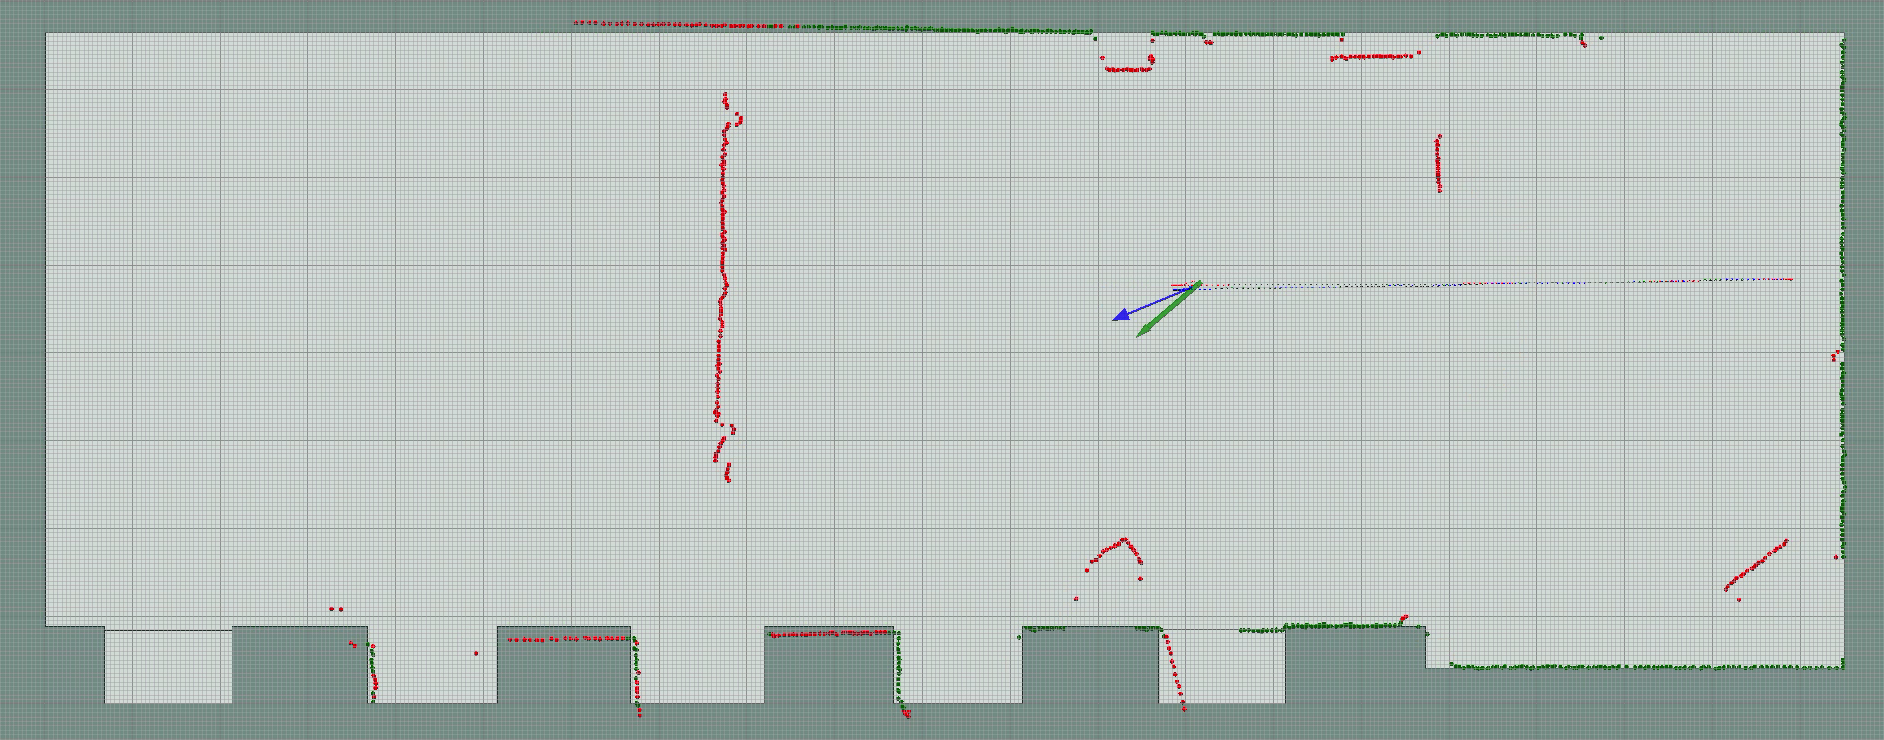
\includegraphics[width=0.47\textwidth]{localization-system-evaluation/tests-3dof/laser-spherical-interpolation/laser-deformation-1}
	\caption{Large laser deformation on opposite walls when the robot is rotating}
	\label{fig:localization-system-evaluation_laser-deformation-1}
\end{figure}

\begin{figure}[ht]
	\centering
	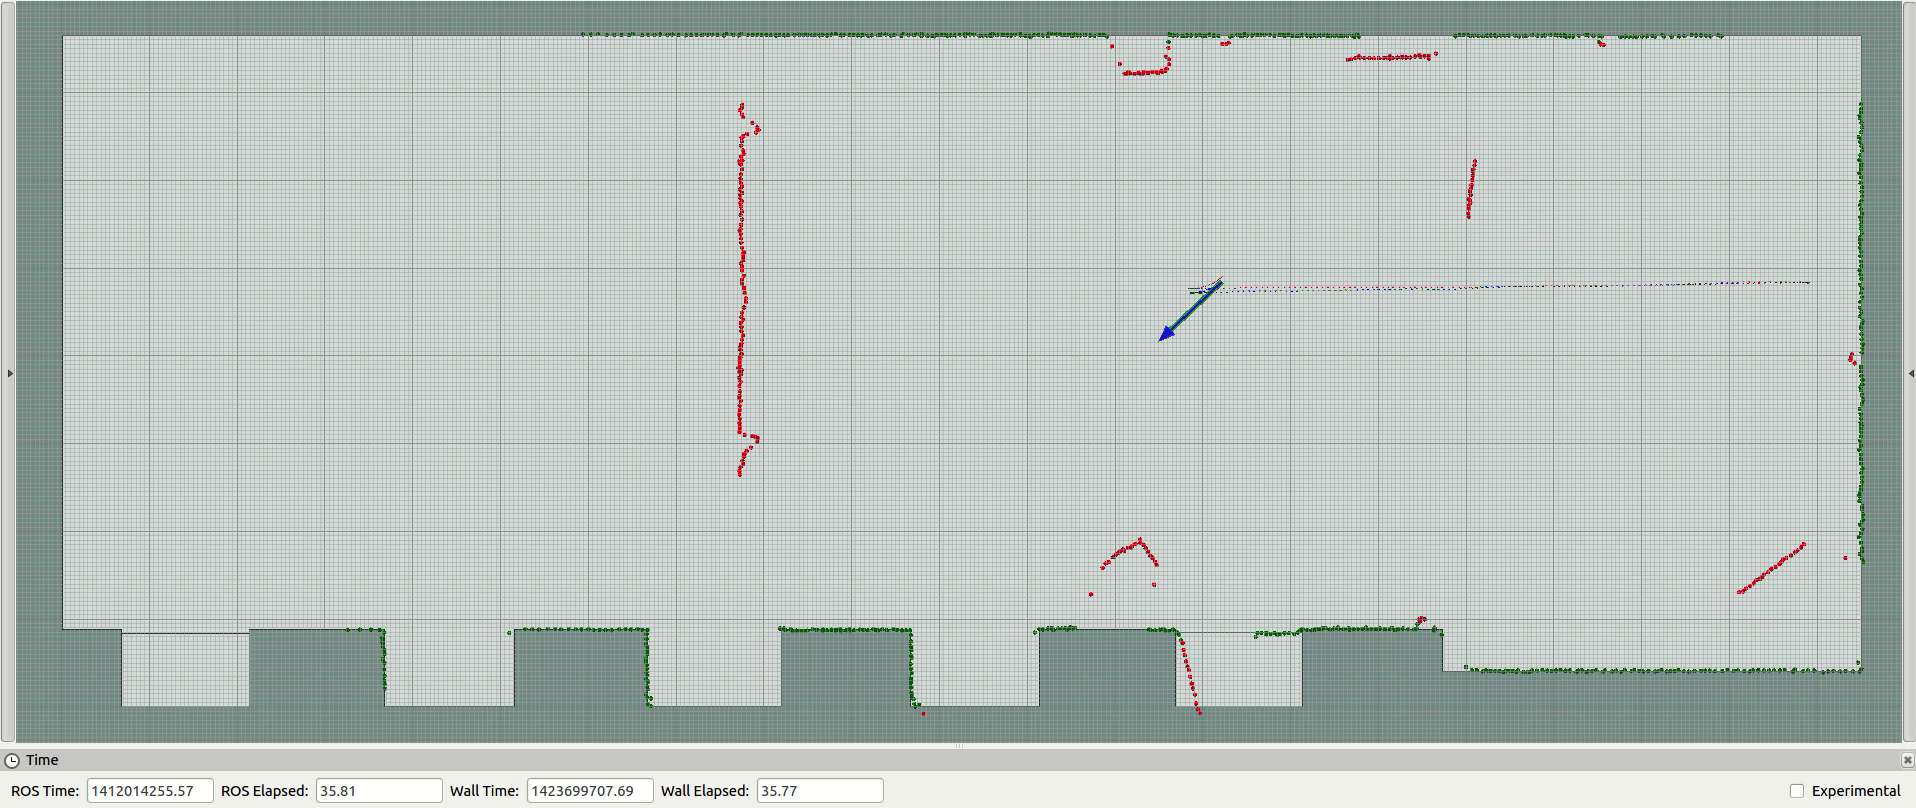
\includegraphics[width=0.47\textwidth]{localization-system-evaluation/tests-3dof/laser-spherical-interpolation/laser-deformation-1-corrected}
	\caption{Correction of the large laser deformation on opposite walls with spherical linear interpolation}
	\label{fig:localization-system-evaluation_laser-deformation-1-corrected}
\end{figure}


\begin{figure}[ht]
	\centering
	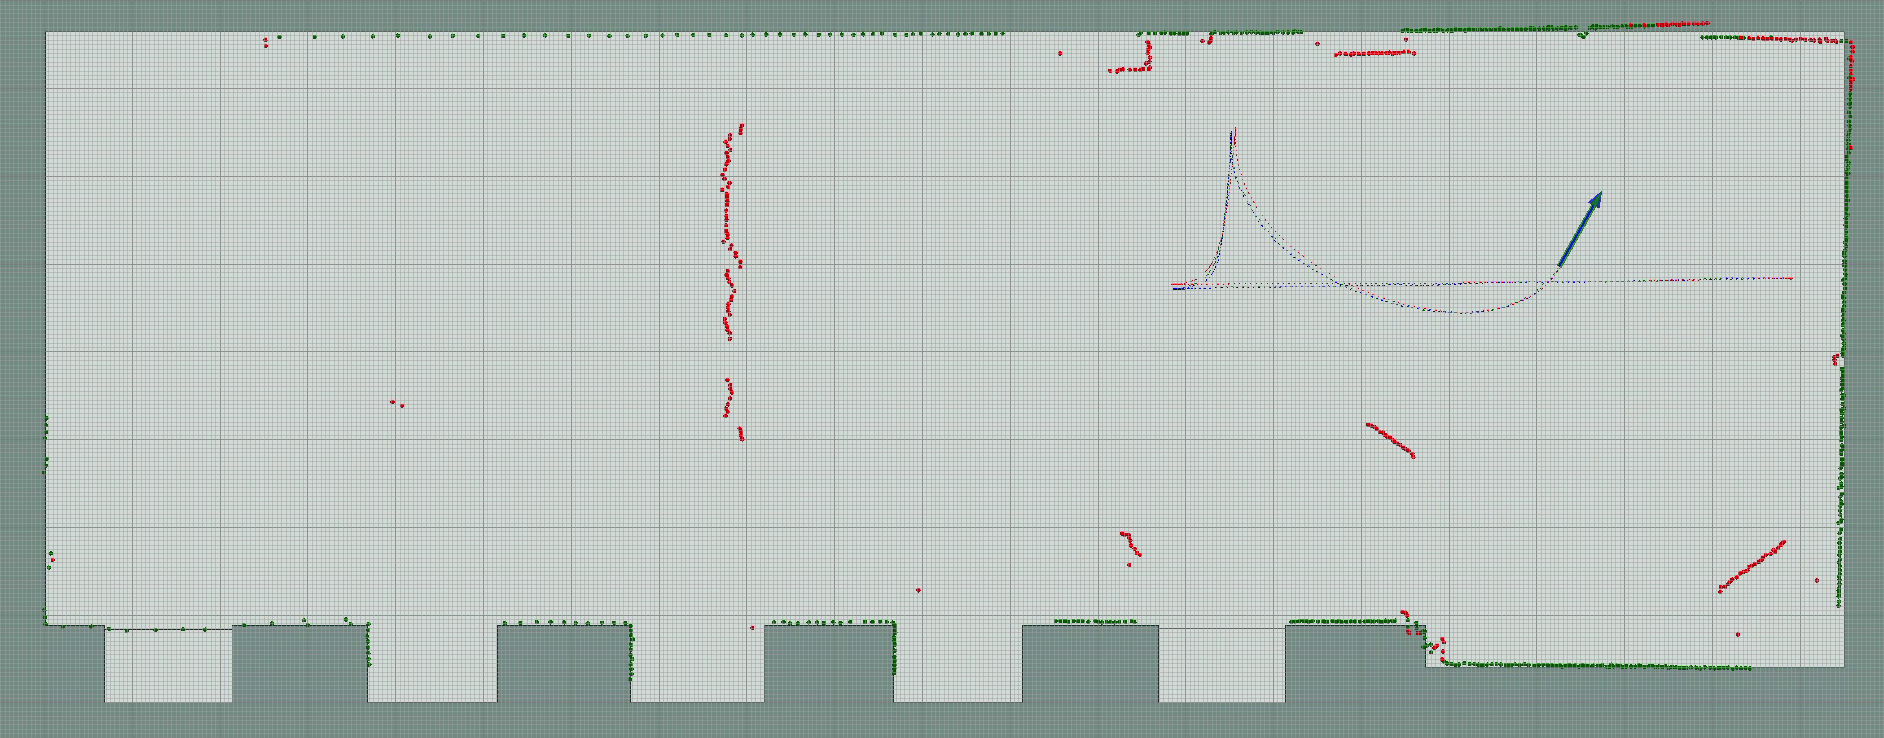
\includegraphics[width=0.47\textwidth]{localization-system-evaluation/tests-3dof/laser-spherical-interpolation/laser-deformation-2}
	\caption{Laser deformation when the robot is rotating}
	\label{fig:localization-system-evaluation_laser-deformation-2}
\end{figure}

\begin{figure}[ht]
	\centering
	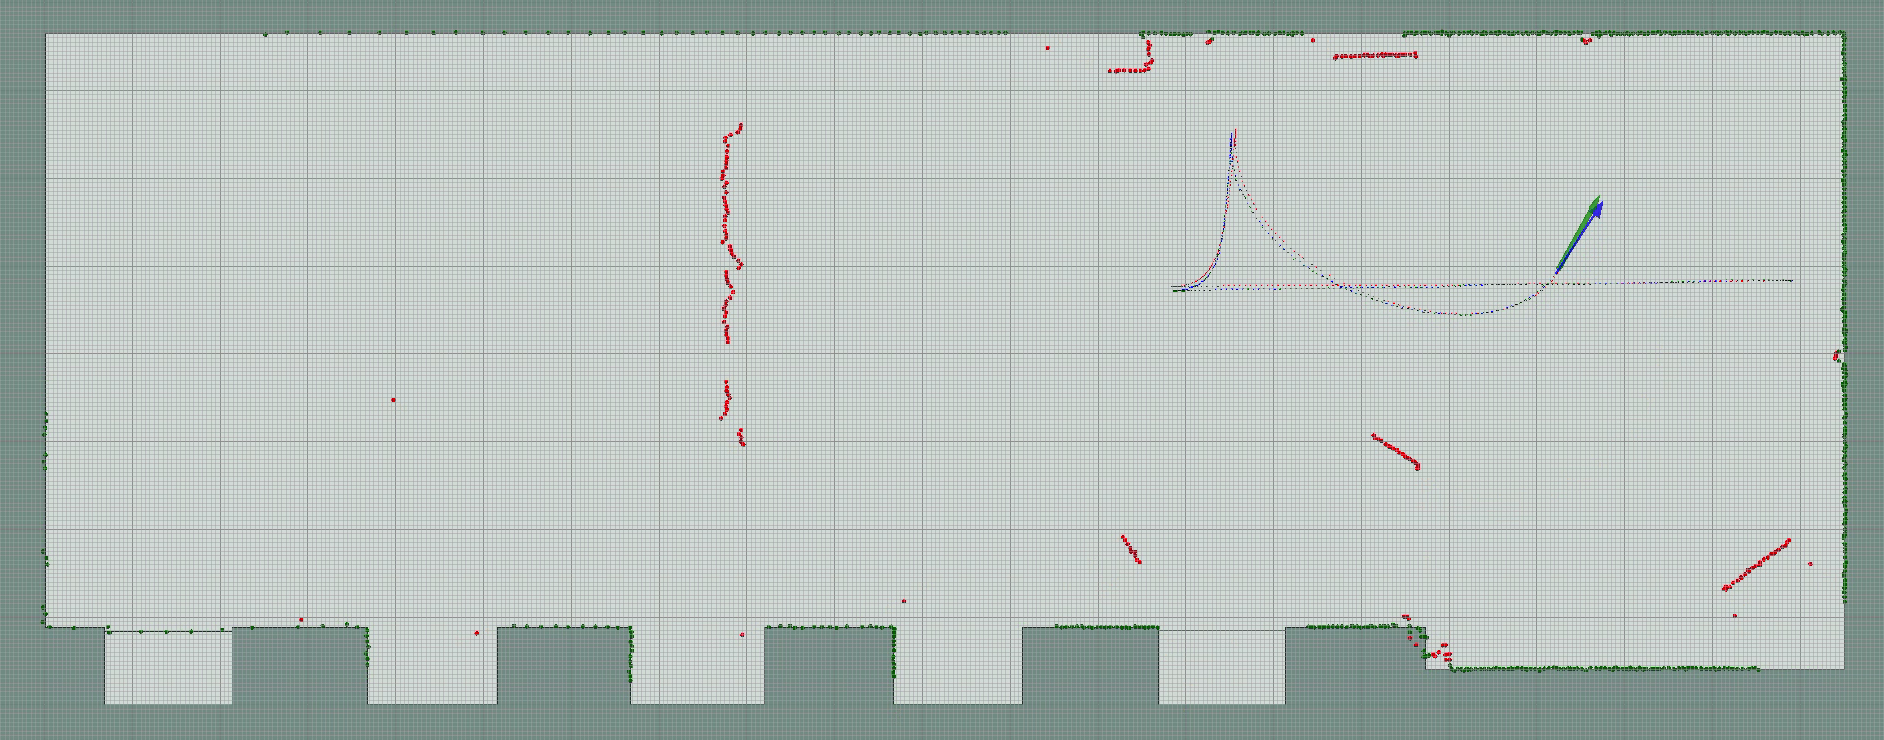
\includegraphics[width=0.47\textwidth]{localization-system-evaluation/tests-3dof/laser-spherical-interpolation/laser-deformation-2-corrected}
	\caption{Correction of the laser deformation with spherical linear interpolation}
	\label{fig:localization-system-evaluation_laser-deformation-2-corrected}
\end{figure}



\subsection{Point cloud preprocessing}

The statistical error of the lasers can be mitigated by merging several laser scans before performing a point cloud registration. This is based on the fact that a considerable amount of laser noise follows a Gaussian distribution, and as such, the effective measurement error can be significantly reduced by retrieving the centroids of a voxel grid applied over the laser data. However, assembling too much laser scans can lead to worse pose tracking if the robot is moving at high speeds, because the lasers would be projected into the map frame with a high position error (because odometry accuracy decreases when the robot speed increases and the localization system will not correct it). As such, the implemented laser assembler supports dynamic reconfiguration of the number of laser scans to assemble (or the period of assembly time) based on the robot estimated velocity. This feature besides improving the pose tracking, it also allows a navigation supervisor to regulate the rate at which the localization system operates. This can be very useful for mobile manipulators because the localization system can have a high update rate when the robot is moving fast and a low update rate when it is moving slower or when it is stopped. This allows a more efficient usage of the platform hardware resources while also improving the localization system accuracy.

Besides reducing the sensor measurement errors, this processing stage also allows the removal of laser shadow points caused by veiling, or small cluster of points that may be associated with temporary objects / people. Moreover, given that the time it takes to perform point cloud registration is proportional to the number of points in the reference and ambient point cloud, voxel / random downsampling can be very effective techniques to adjust the level of detail required (given the computational resources available).



\subsection{\glsentrytext{slam}}

Any self-localization system requires a map to estimate the pose of the robot when using exteroceptive information. If such map doesn't exist, then the first point cloud can be considered as the initial map, and then it can be updated dynamically as new sensor data is processed. This map update approach can use the full registered point cloud or the inliers / outliers only. Full integration is useful when starting a map from scratch (example in \cref{fig:localization-system-evaluation_drl-2.5cm-1.0-bag-speed}). Partial integration can be useful when there is a highly detailed map and we only want to add or remove information from it (examples from \crefrange{fig:localization-system-evaluation_lab-10mm}{fig:localization-system-evaluation_indoor-10mm-dynamic}). Partial integration besides reducing the computational resources required it also allows to keep the detail of the source map, avoiding deformations due to sensor measurement noise. This noise is noticeable in the walls of the map in \cref{fig:localization-system-evaluation_lab-10mm-dynamic} (updated with full integration) and was avoided in the map in \cref{fig:localization-system-evaluation_indoor-10mm-dynamic} (updated with outliers only).

Looking at figures from \crefrange{fig:localization-system-evaluation_drl-2.5cm-1.0-bag-speed}{fig:localization-system-evaluation_ground-truth-2.5cm-0.245-time-offset} it can be seen that the proposed localization system was able to achieve equal or even better mapping results than the GMapping\footnote{\url{http://wiki.ros.org/gmapping}} \gls{slam} system and even the ground truth provided by the Raptor-E cameras (that seems to be less suitable for mapping than both the proposed localization system and the GMapping \gls{ros} package).


\begin{figure}[H]
	\centering
	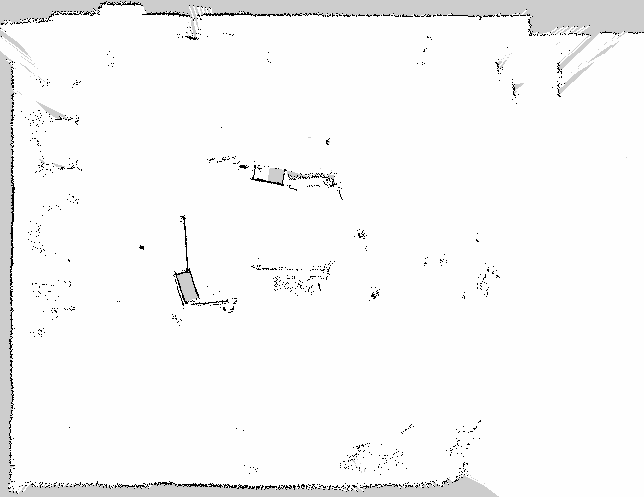
\includegraphics[width=0.33\textwidth]{localization-system-evaluation/tests-3dof/maps/industrial-hall/drl-2.5cm-1.0-bag-speed}
	\caption{Map made with the localization system using full integration in conjunction with OctoMap}
	\label{fig:localization-system-evaluation_drl-2.5cm-1.0-bag-speed}
\end{figure}

\begin{figure}[H]
	\centering
	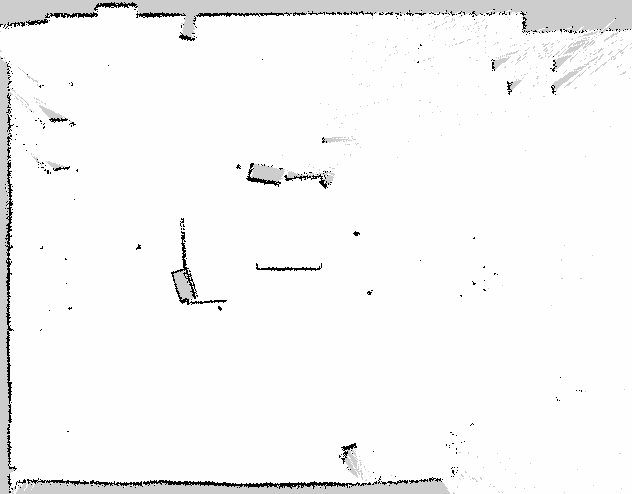
\includegraphics[width=0.33\textwidth]{localization-system-evaluation/tests-3dof/maps/industrial-hall/gmapping-2.5cm-0.1-bag-speed}
	\caption{Map made with the GMapping package playing the rosbag at 10\% speed}
	\label{fig:localization-system-evaluation_gmapping-2.5cm-0.1-bag-speed}
\end{figure}

\begin{figure}[H]
	\centering
	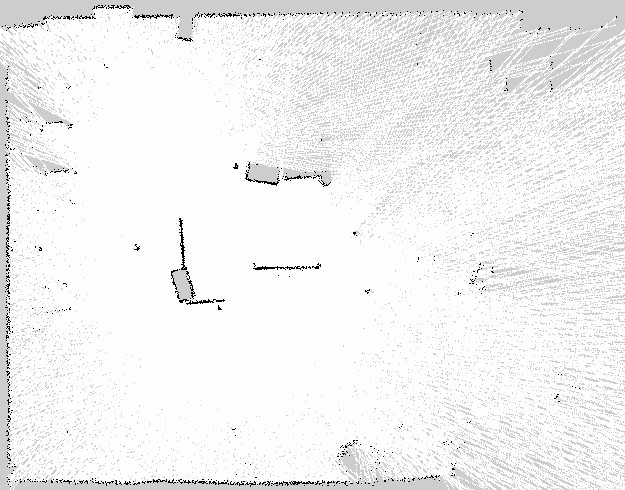
\includegraphics[width=0.27\textwidth]{localization-system-evaluation/tests-3dof/maps/industrial-hall/gmapping-2.5cm-1.0-bag-speed}
	\caption{Map made with the GMapping package playing the rosbag in real time}
	\label{fig:localization-system-evaluation_gmapping-2.5cm-1.0-bag-speed}
\end{figure}

\begin{figure}[H]
	\centering
	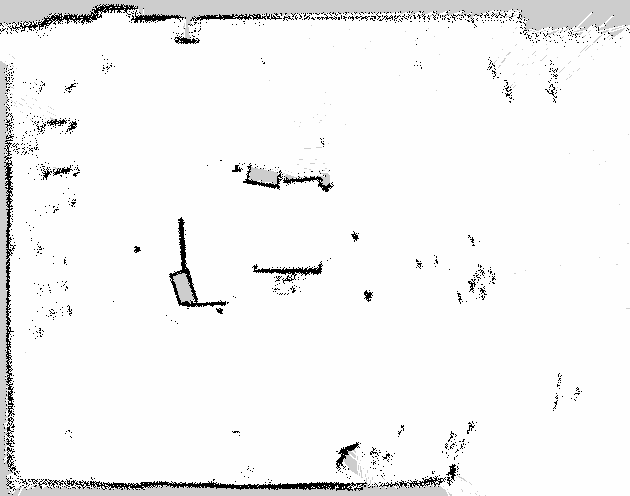
\includegraphics[width=0.27\textwidth]{localization-system-evaluation/tests-3dof/maps/industrial-hall/ground-truth-2.5cm-0.245-time-offset}
	\caption{Map made using the ground truth poses provided by the Raptor-E cameras}
	\label{fig:localization-system-evaluation_ground-truth-2.5cm-0.245-time-offset}
\end{figure}


\begin{figure}[H]
	\centering
	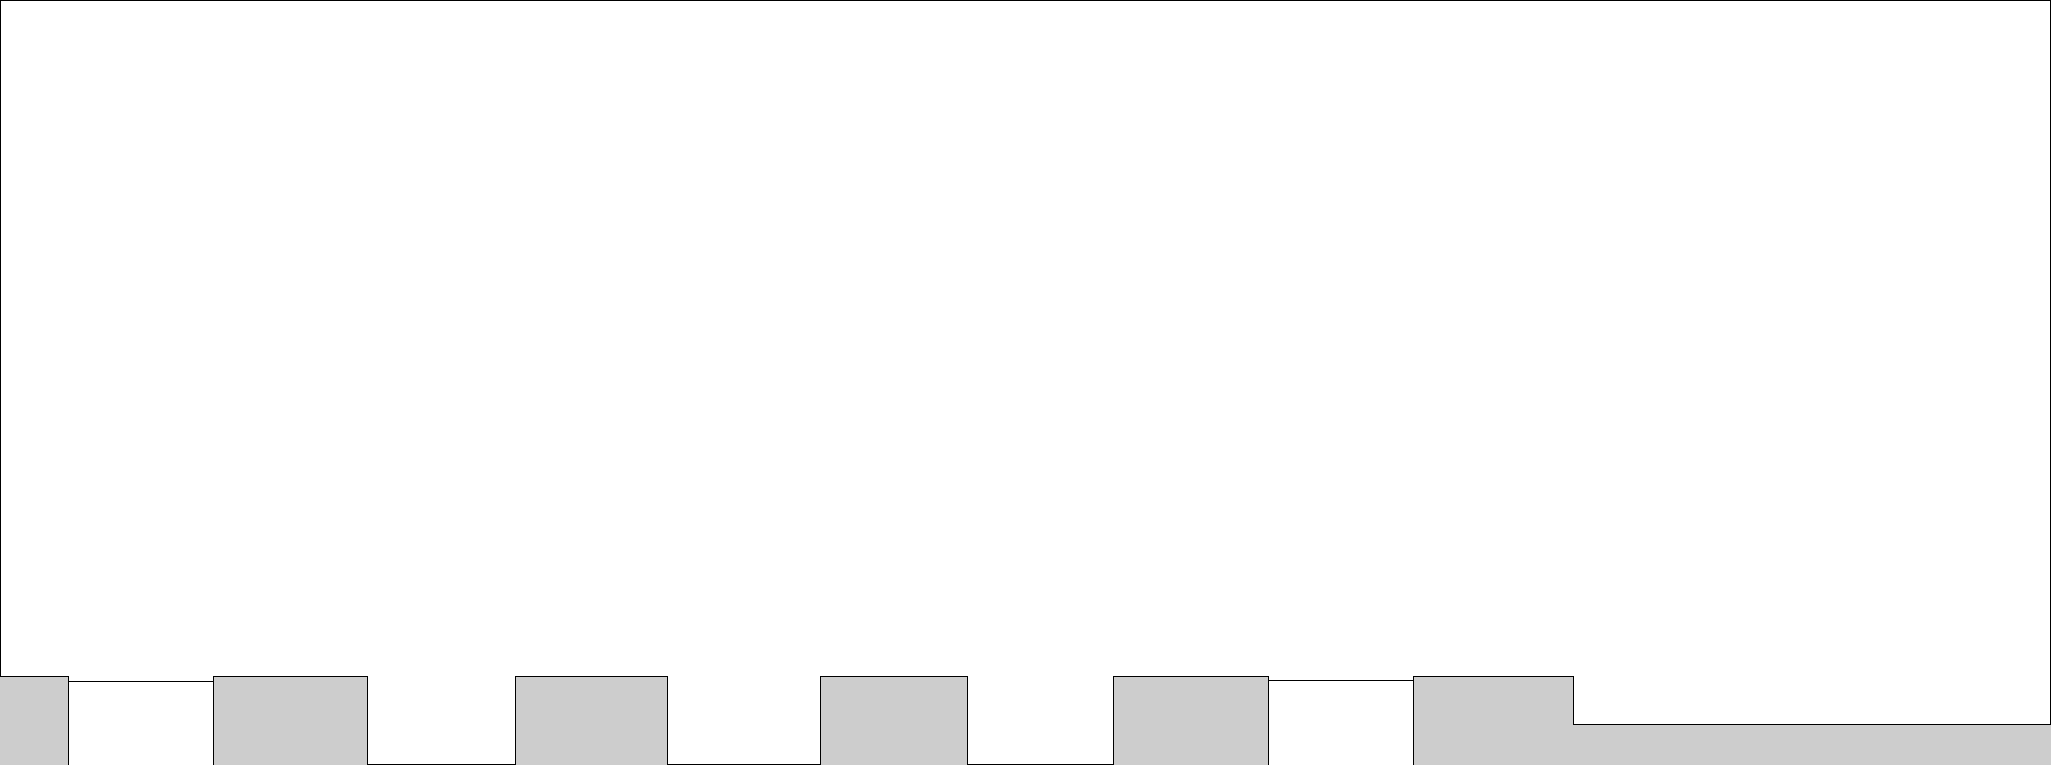
\includegraphics[width=0.27\textwidth]{localization-system-evaluation/tests-3dof/maps/lab-10mm}
	\caption{Original map from RoboCup field}
	\label{fig:localization-system-evaluation_lab-10mm}
\end{figure}

\begin{figure}[H]
	\centering
	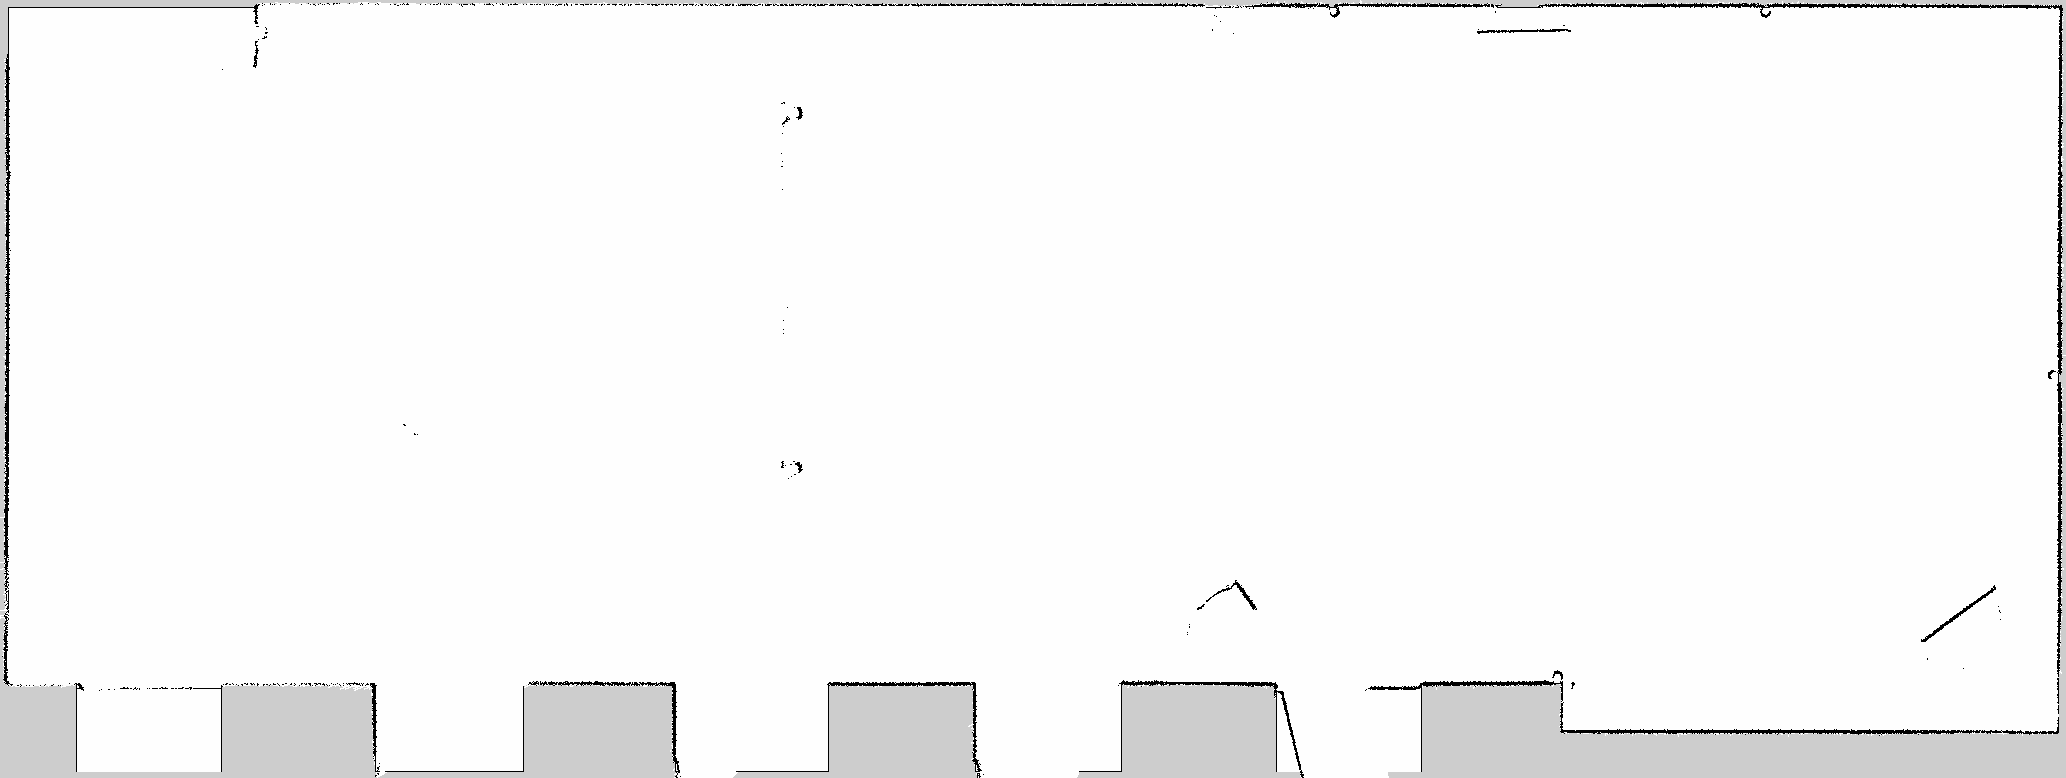
\includegraphics[width=0.27\textwidth]{localization-system-evaluation/tests-3dof/maps/lab-10mm-dynamic}
	\caption{Updated map of RoboCup field using full integration}
	\label{fig:localization-system-evaluation_lab-10mm-dynamic}
\end{figure}

\begin{figure}[H]
	\centering
	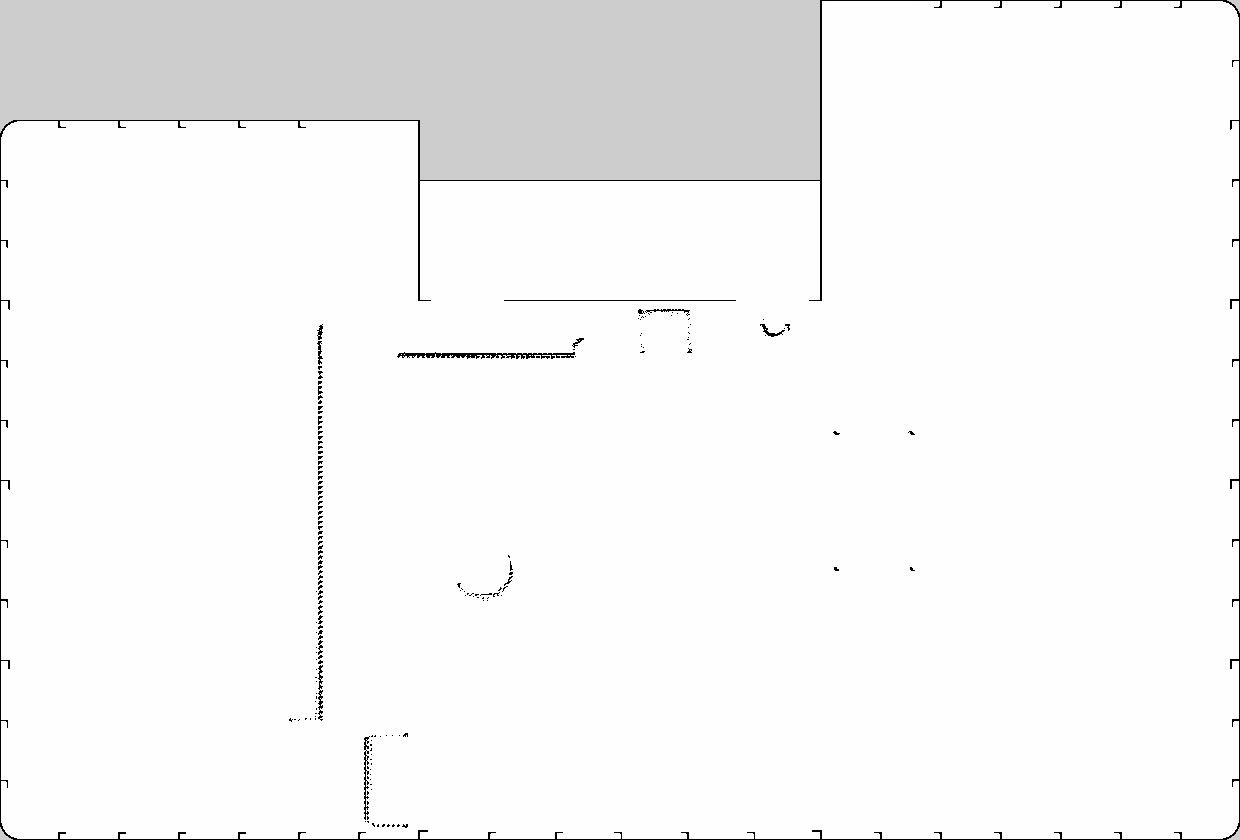
\includegraphics[width=0.27\textwidth]{localization-system-evaluation/tests-3dof/maps/indoor-10mm-dynamic}
	\caption{Updated map of structured environment using partial integration (only points that were not close to the walls were integrated)}
	\label{fig:localization-system-evaluation_indoor-10mm-dynamic}
\end{figure}



\subsection{Point cloud registration}

Looking at the results from \cref{tab:localization-system-evaluation_3-dof-results,tab:localization-system-evaluation_3-dof-results-odometry-amcl}, the poses from \cref{fig:localization-system-evaluation_complex-path-with-outliers-50-30-50-10cm-per-sec-velocity-1-4-scans-paths}, the laser assembly figures shown in \cref{fig:localization-system-evaluation_complex-path-with-outliers-50-30-50-10cm-per-sec-velocity-1-4-scans-drl-cumulative,fig:localization-system-evaluation_complex-path-with-outliers-50-30-50-10cm-per-sec-velocity-1-4-scans-amcl-cumulative} and the translation / rotation error graphs presented from \crefrange{fig:localization-system-evaluation_complex-path-with-outliers-50-30-50-10cm-per-sec-velocity-1-4-translation-error-amcl}{fig:localization-system-evaluation_complex-path-with-outliers-50-30-50-10cm-per-sec-velocity-1-4-rotation-error} (from the Jarvis test in the complex path at high velocities), it can be seen that the localization system can registered point clouds with much more accuracy than \gls{amcl} (even when using over 5000 particles). The only problems that seem to affect the registration algorithms are the point cloud deformation (usually when there is unreliable odometry information, which typically occurs when the robot is moving with high velocities / accelerations), laser measurements errors, unknown objects close to the known reference point cloud and also low resolution maps.

The localization system can tolerate these problems by having a default pipeline configuration for the normal operation of the robot, another for temporary tracking recovery and yet another for initial pose estimation.

The switch between the localization system operation modes using the point cloud registration analysis proved to be a very intuitive and fast process and the overall system configurations seemed to be generic enough to be reused in several types of environments, with different robots equipped with varying types of sensors. Such ease of configuration allows the fast deployment of robots and gives a high confidence that the localization system will remain accurate even in challenging environments. This is not the case with systems such as \gls{amcl}, given that they are very dependent on the odometry and laser models, and as such, require constant retuning when one of these models change.

The ability to switch registration algorithms at runtime based on the quality of the estimated pose proved to be an efficient and flexible architecture choice, since it allowed high precision pose tracking with fast registration algorithms and occasional pose tracking recovery with more robust methods / configurations (which happened more often in the tests at higher velocities, in which the odometry was significantly worse).

The initial pose estimation using feature matching was very reliable and successfully found the robot location even in low feature surroundings (as can be seen in \cref{fig:localization-system-evaluation_ship-interior-initial-pose-estimation-sift-fpfh-ransac-gicp,fig:localization-system-evaluation_jarvis-initial-pose-estimation-sift-fpfh-ransac-gicp-1}). Moreover, the output of the accepted initial pose estimations allows the detection of similar map locations by a navigation supervisor, which can then plot a path to disambiguate the initial pose guess and avoid dangerous operations at a wrong position.

\Cref{fig:localization-system-evaluation_ship-interior-initial-pose-estimation-sift-fpfh-ransac-gicp,fig:localization-system-evaluation_jarvis-initial-pose-estimation-sift-fpfh-ransac-gicp-1} show the accepted initial pose estimations using the global localization subsystem presented in \cref{subsec:localization-system_feature-registration}.

The blue circles presented in \cref{fig:localization-system-evaluation_jarvis-initial-pose-estimation-sift-fpfh-ransac-gicp-1} represent the keypoints of the ambient point cloud in the robot start up position, while the violet circles are the reference point cloud keypoints. The green circles are the ambient point cloud laser measurements after performing the initial pose estimation and registration refinement.


\begin{figure}[H]
	\centering
	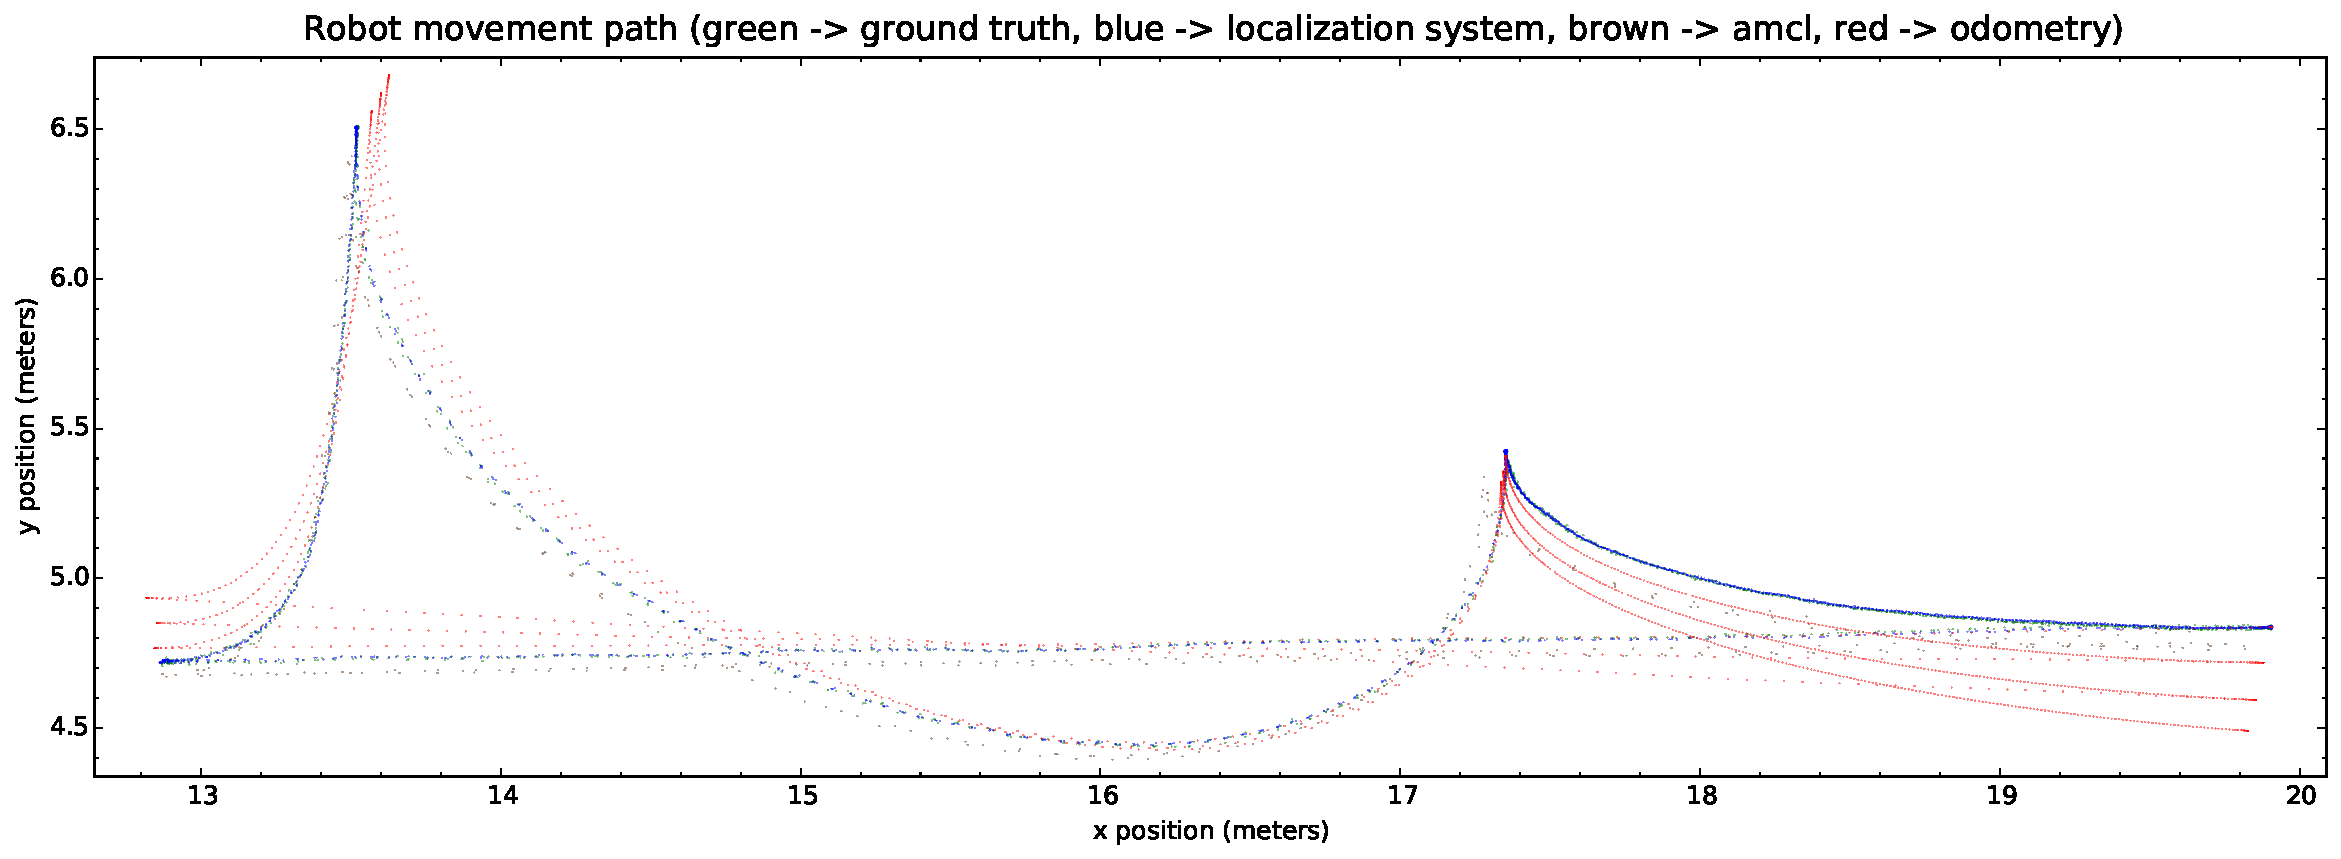
\includegraphics[width=0.42\textwidth]{localization-system-evaluation/tests-3dof/jarvis-robot/complex-path-with-outliers-50-30-50-10cm-per-sec-velocity-1-4-scans/graphs/robot-movement-path-with-odometry-and-amcl}
	\caption{Poses estimated by the ground truth, localization system, \glsentrytext{amcl} and odometry}
	\label{fig:localization-system-evaluation_complex-path-with-outliers-50-30-50-10cm-per-sec-velocity-1-4-scans-paths}
\end{figure}

\begin{figure}[H]
	\centering
	\includegraphics[width=0.37\textwidth]{localization-system-evaluation/tests-3dof/jarvis-robot/complex-path-with-outliers-50-30-50-10cm-per-sec-velocity-1-4-scans/drl-cumulative}
	\caption{Laser scans assembled on top of the map using the localization system poses}
	\label{fig:localization-system-evaluation_complex-path-with-outliers-50-30-50-10cm-per-sec-velocity-1-4-scans-drl-cumulative}
\end{figure}

\begin{figure}[H]
	\centering
	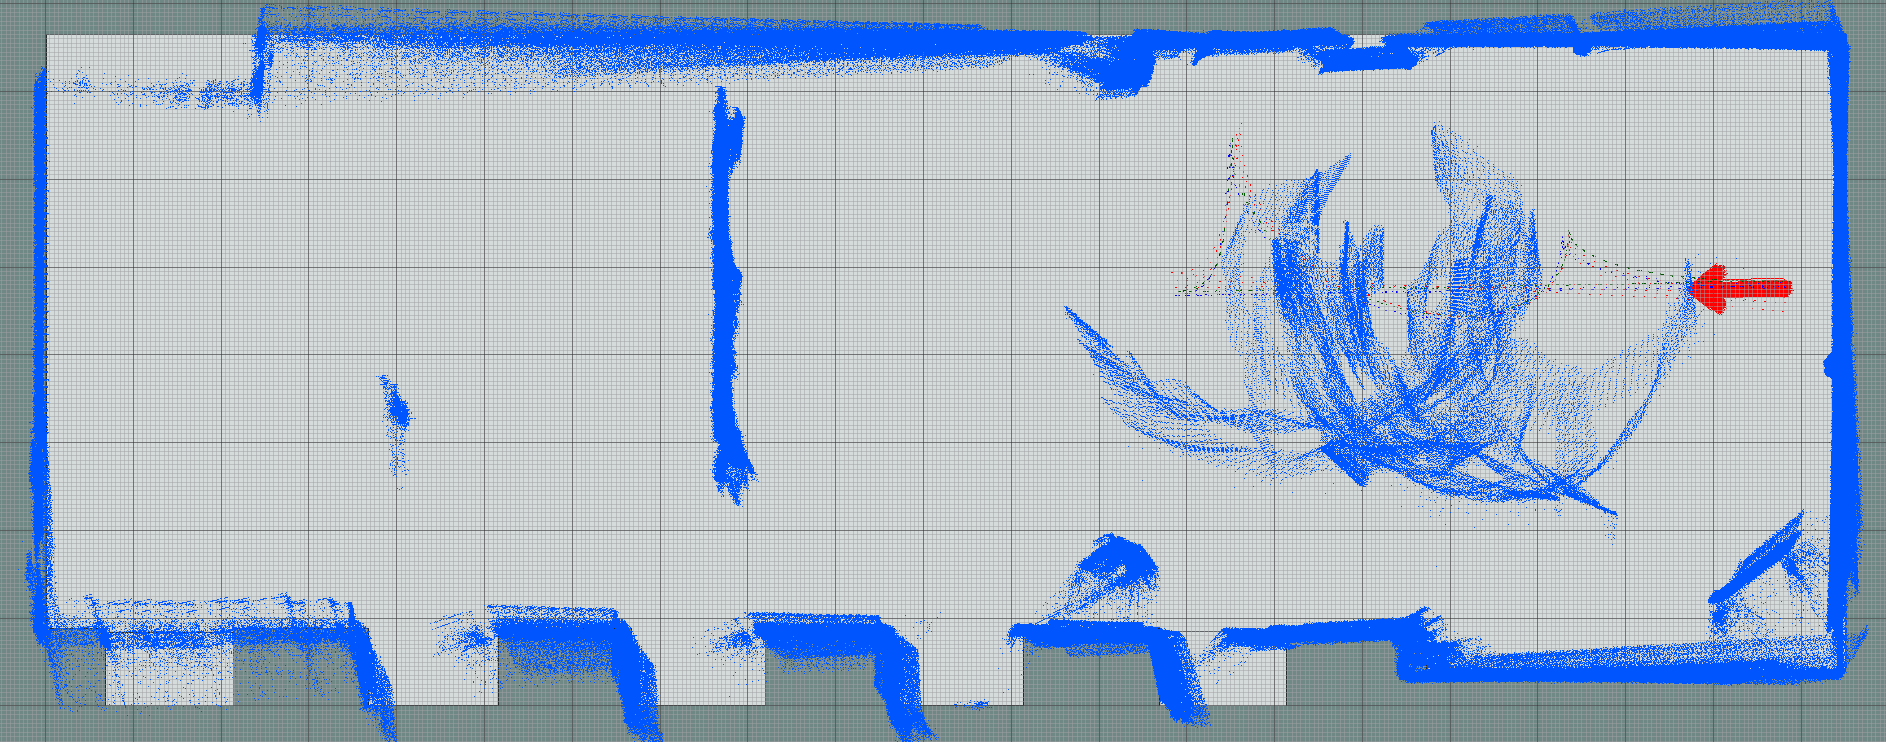
\includegraphics[width=0.37\textwidth]{localization-system-evaluation/tests-3dof/jarvis-robot/complex-path-with-outliers-50-30-50-10cm-per-sec-velocity-1-4-scans/amcl-cumulative}
	\caption{Laser scans assembled on top of the map using the \glsentrytext{amcl} poses}
	\label{fig:localization-system-evaluation_complex-path-with-outliers-50-30-50-10cm-per-sec-velocity-1-4-scans-amcl-cumulative}
\end{figure}


\begin{figure}[H]
	\centering
	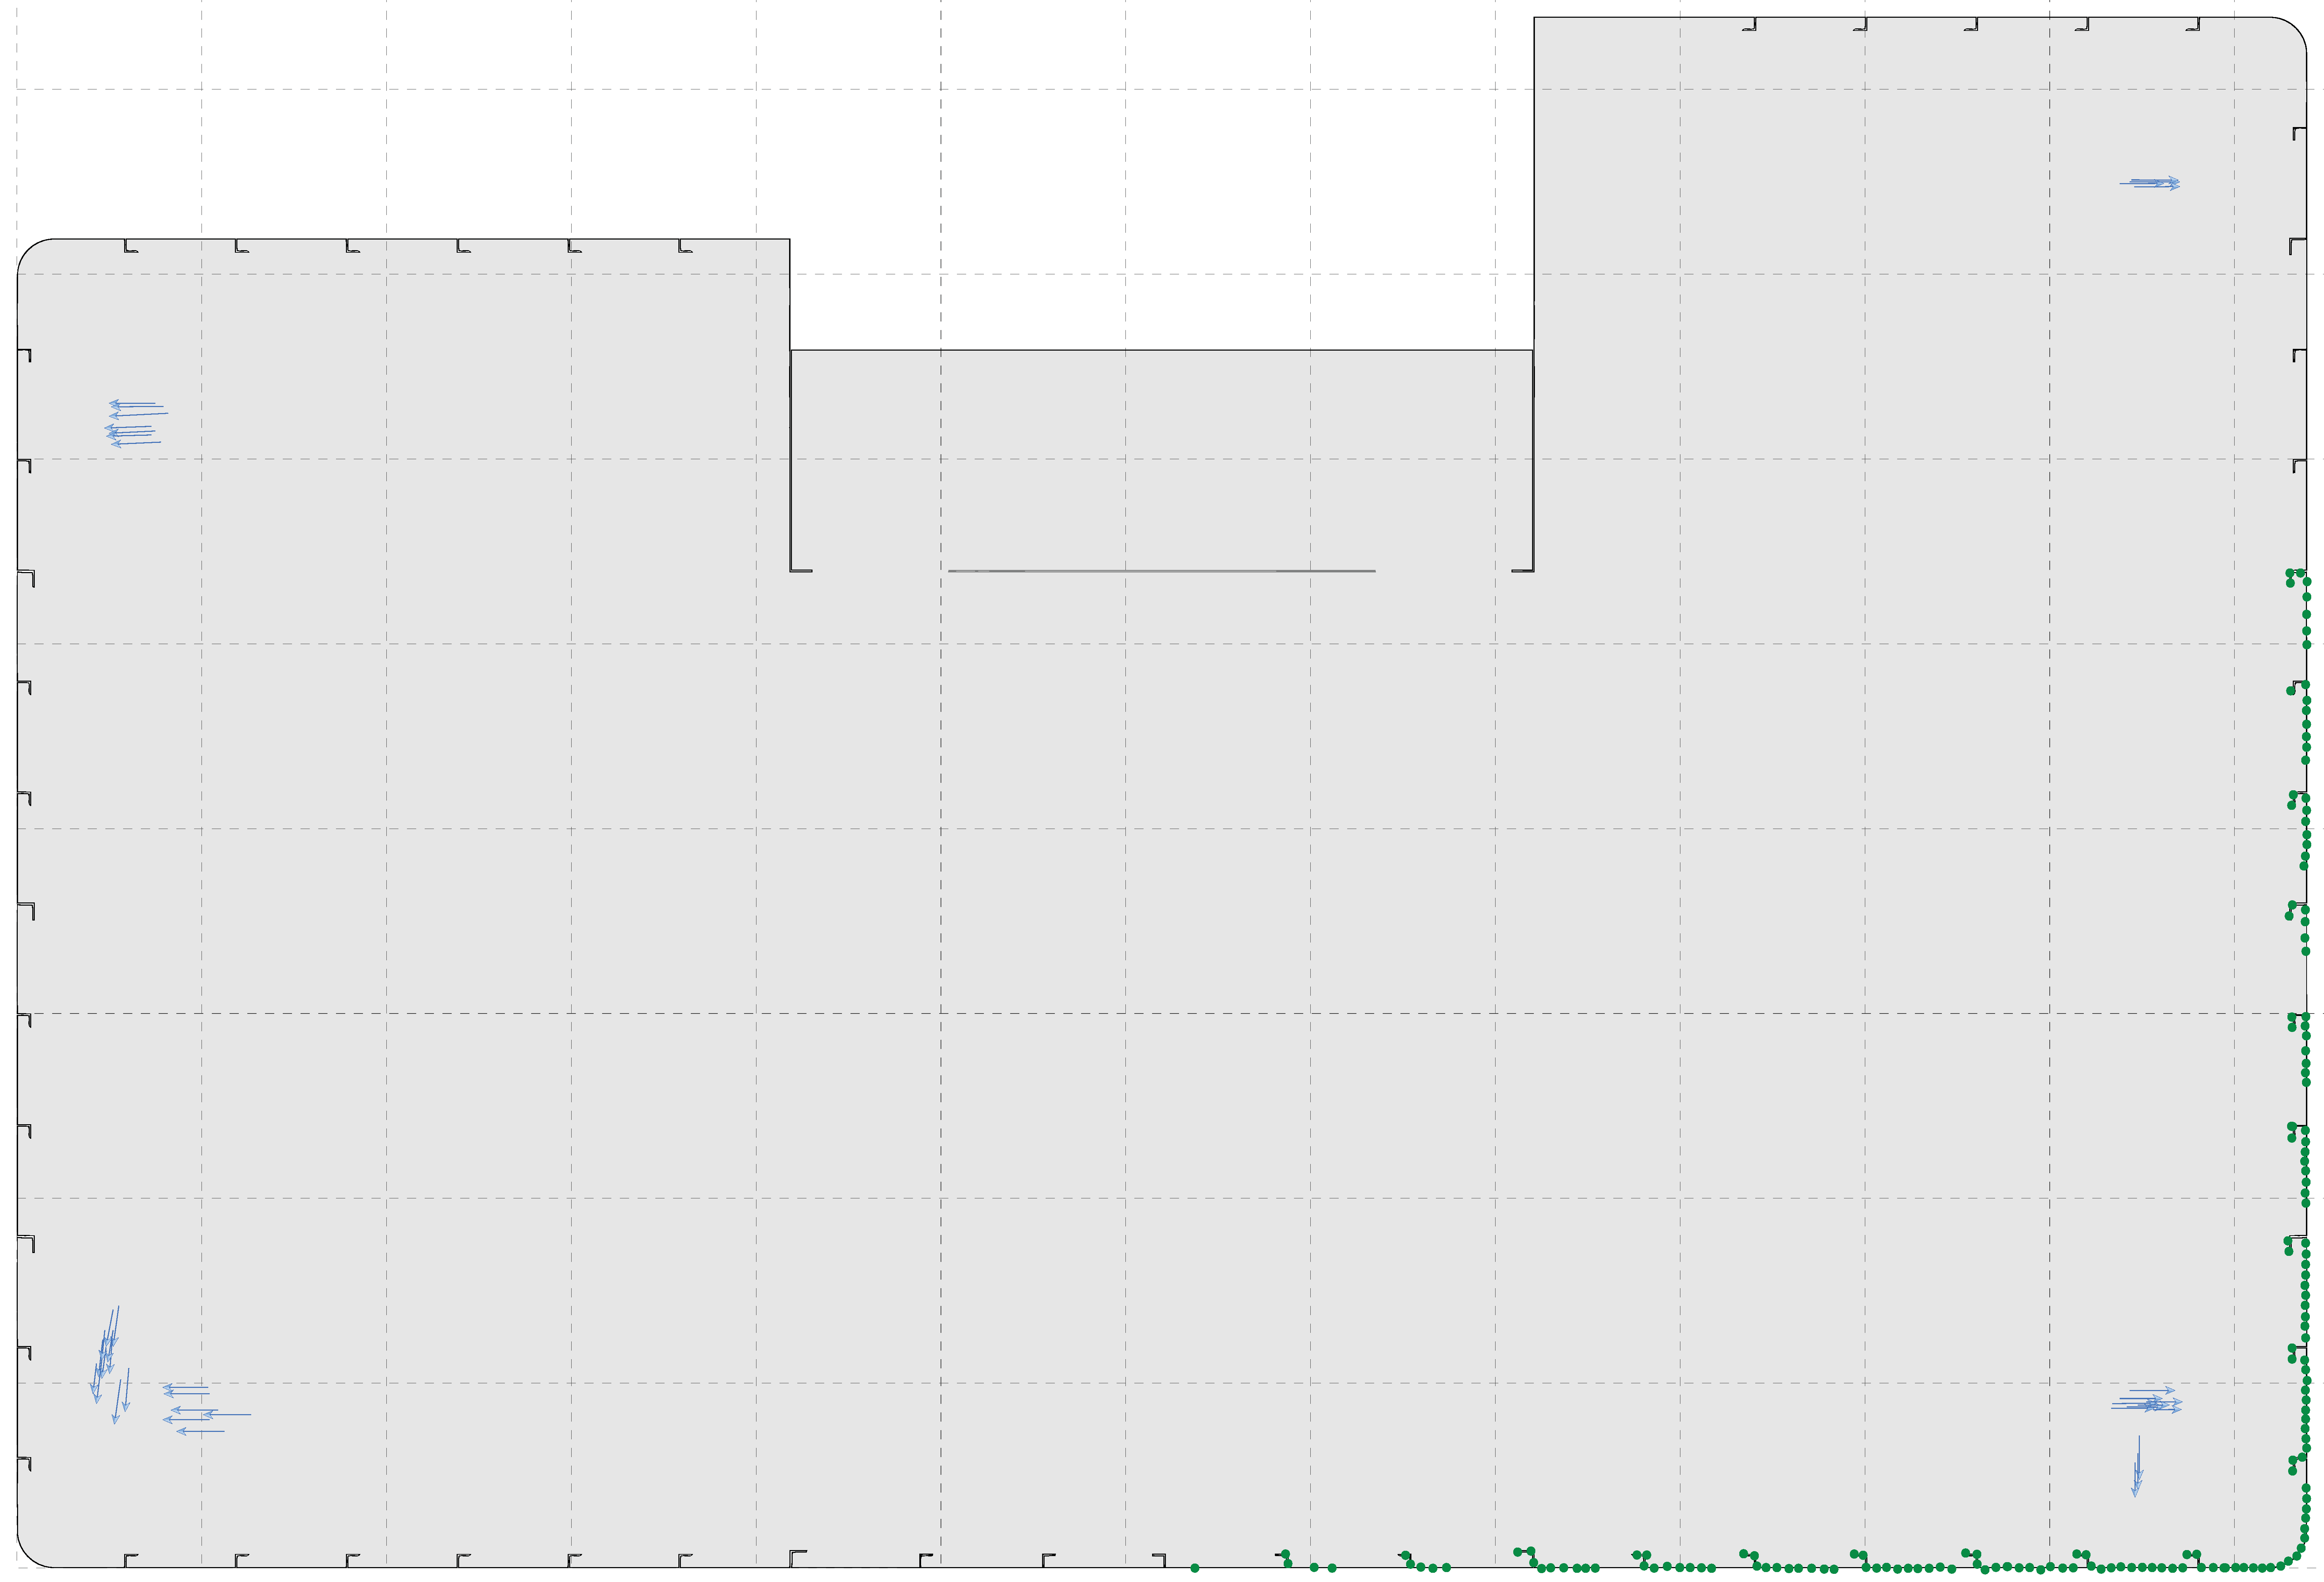
\includegraphics[width=0.3\textwidth]{localization-system-evaluation/tests-3dof/initial_pose_estimation/ship-interior-initial-pose-estimation-sift-fpfh-ransac-gicp}
	\caption{Initial pose estimation using feature matching in Guardian static environment}
	\label{fig:localization-system-evaluation_ship-interior-initial-pose-estimation-sift-fpfh-ransac-gicp}
\end{figure}

\begin{figure}[H]
	\centering
	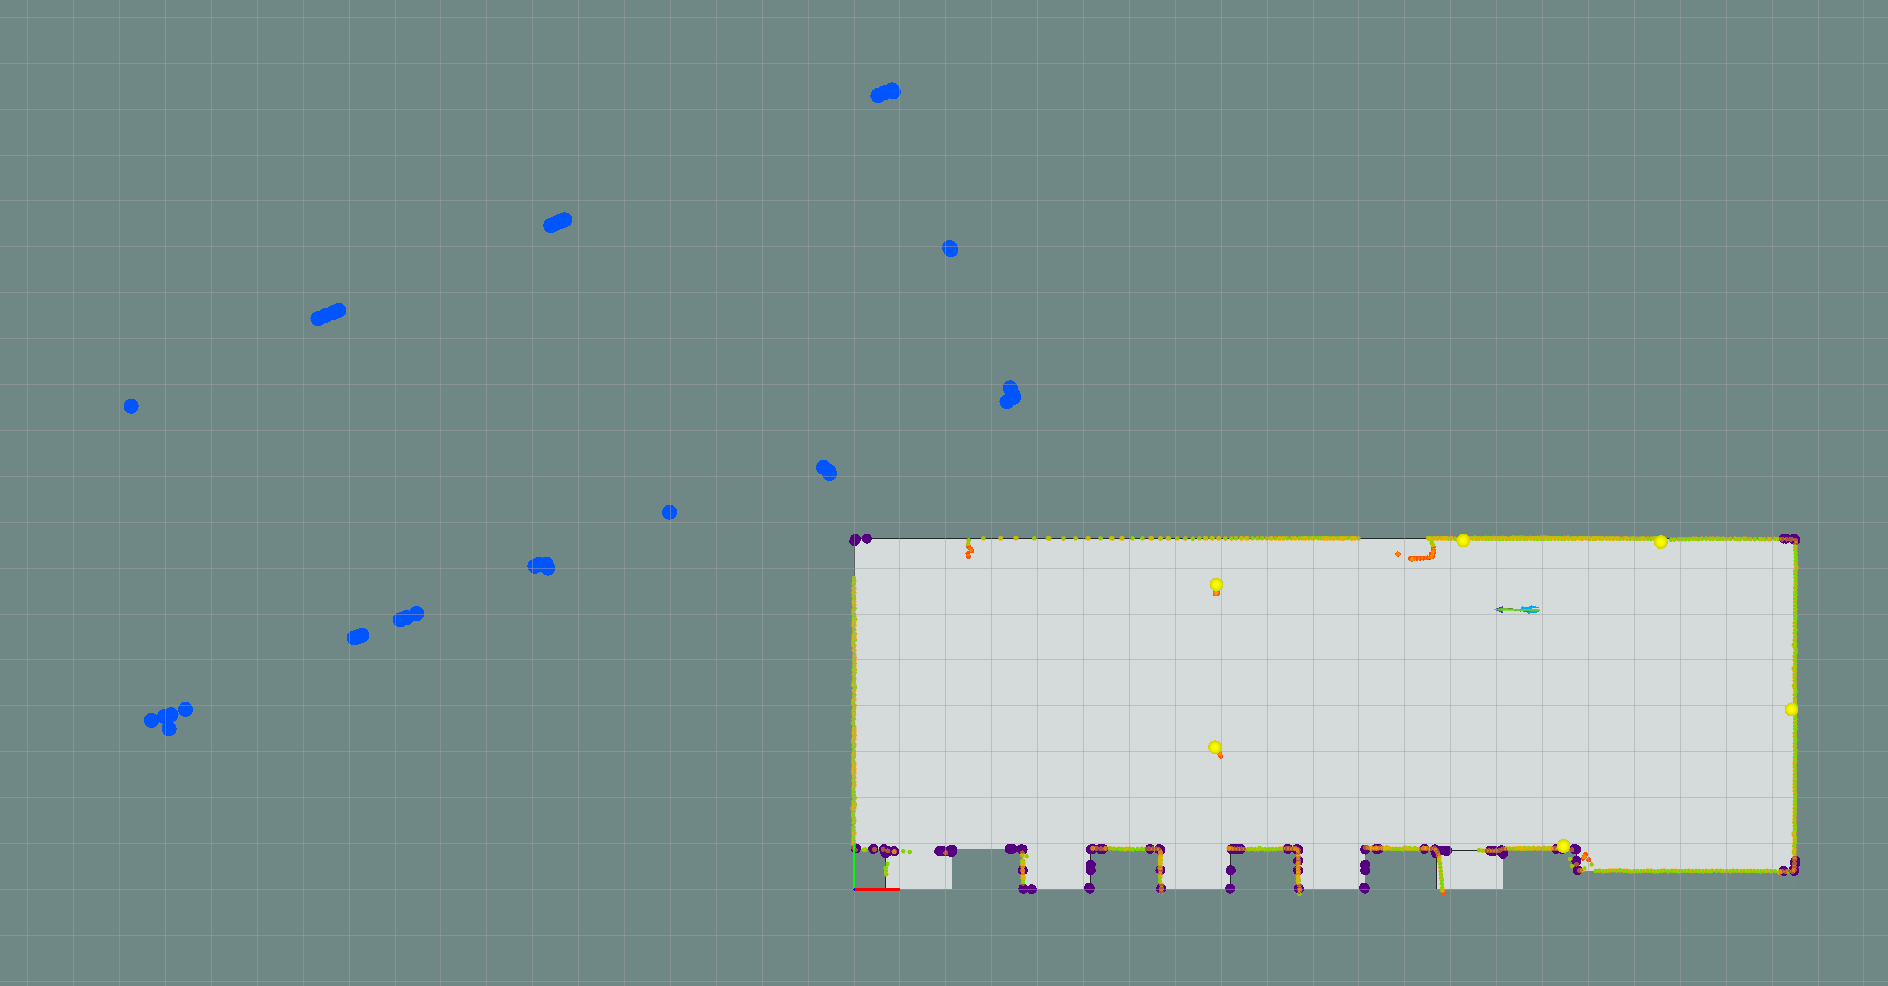
\includegraphics[width=0.3\textwidth]{localization-system-evaluation/tests-3dof/initial_pose_estimation/jarvis-initial-pose-estimation-sift-fpfh-ransac-gicp-1}
	\caption{Initial pose estimation using feature matching in Jarvis environment}
	\label{fig:localization-system-evaluation_jarvis-initial-pose-estimation-sift-fpfh-ransac-gicp-1}
\end{figure}

%\begin{figure}[ht]
%	\centering
%	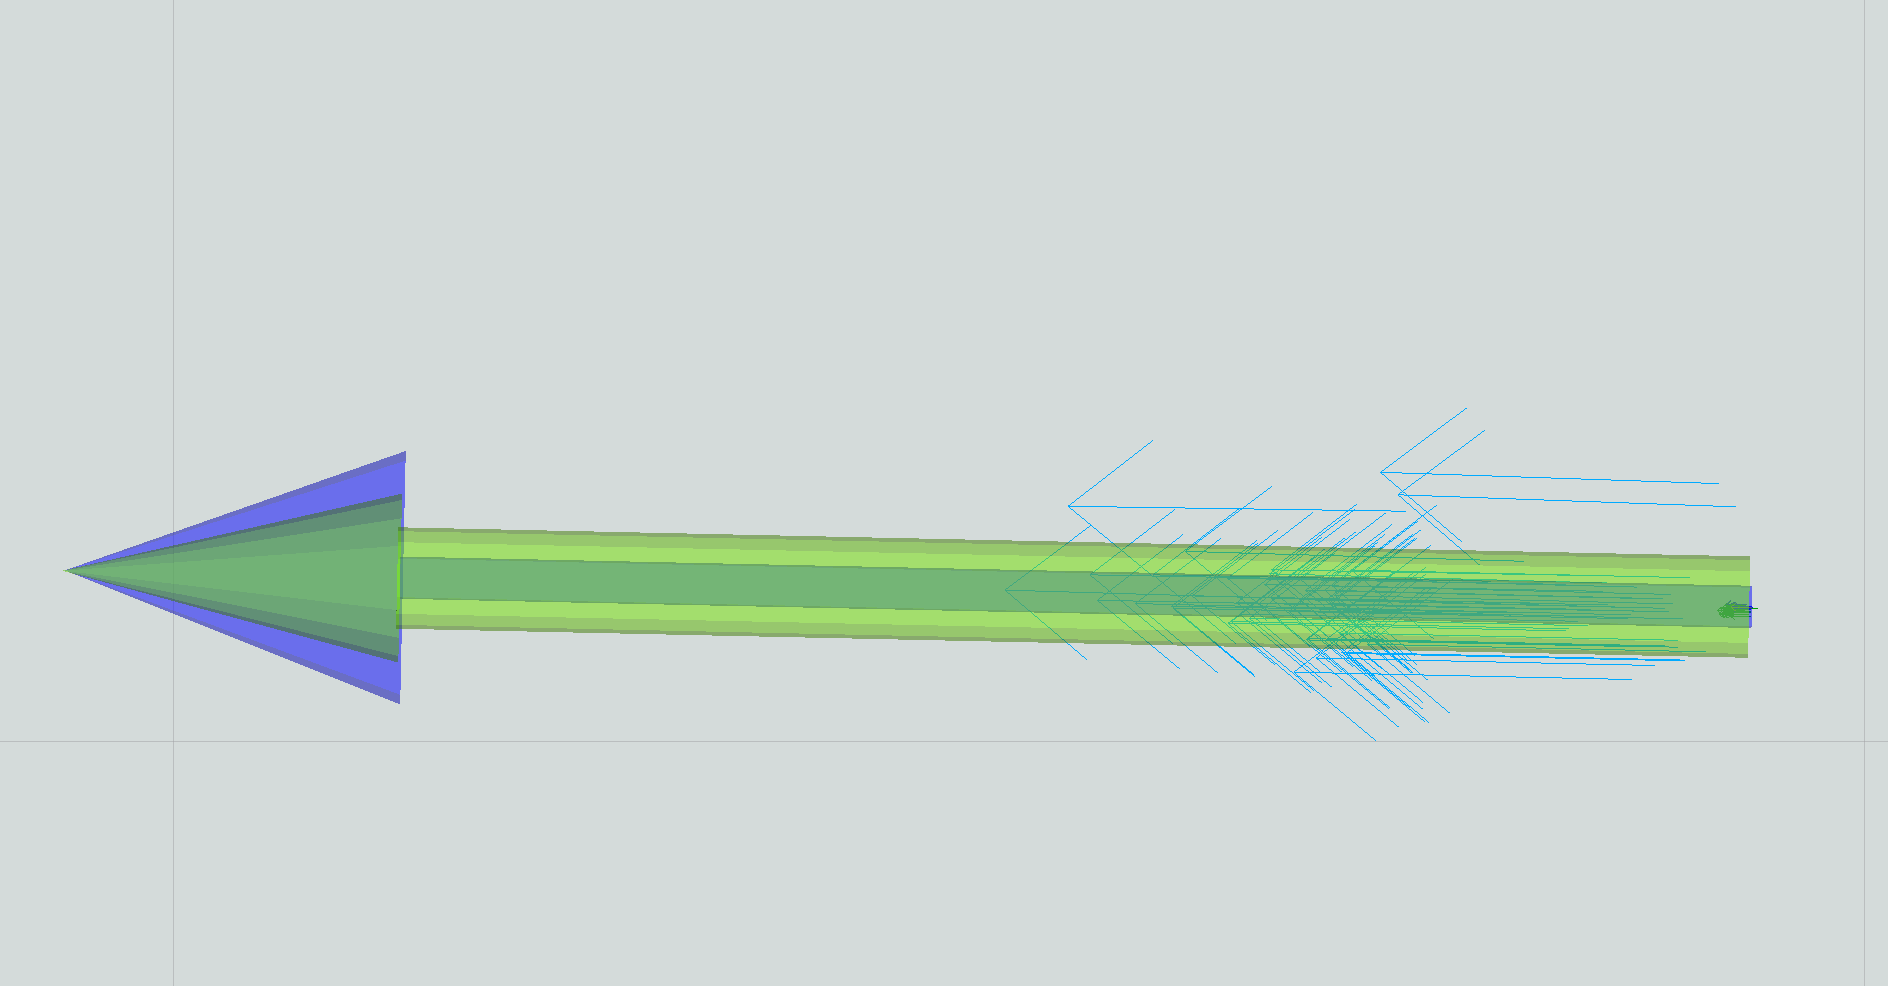
\includegraphics[width=0.2\textwidth]{localization-system-evaluation/tests-3dof/initial_pose_estimation/jarvis-initial-pose-estimation-sift-fpfh-ransac-gicp-2}
%	\caption{Initial pose estimation distribution in Jarvis environment}
%	\label{fig:localization-system-evaluation_jarvis-initial-pose-estimation-sift-fpfh-ransac-gicp-2}
%\end{figure}




\subsection{Translation and rotation errors}

By analyzing \cref{tab:localization-system-evaluation_3-dof-results,tab:localization-system-evaluation_3-dof-results-odometry-amcl} it can be seen that the proposed 3 \gls{dof} localization system can achieve pose tracking with less than 1 cm in translation error and less than 1 degree in rotation error.

As expected, the tests at lower velocities had less mean error than the ones at higher speeds while requiring slightly less computation time. Also, the simulator tests had less mean error than the ones performed on the physical platforms. This is due to laser scan deformation that couldn't be simulated and also because the Gazebo simulator was only able to add Gaussian noise to the laser measurements. To compensate these limitations, the error in odometry and laser measurements in simulation was deliberately higher than the expected values for the physical platforms. This explains why the localization system needed more time to perform the pose estimations in the simulator tests. It can also be seen that adding unknown objects increased the mean error and required computation time while adding dynamic objects increased these values even further (given that a moving object appears in a laser scan as a deformed version of its static shape).

Comparing the results of the tests performed with Jarvis robot  with the tests of the Pioneer robot, it can be seen that even when severely reducing the laser range (from 80 to 6 meters), moving the robot in dynamic environments with large occluding objects and even when using a low resolution map (25 mm in the Pioneer tests vs 10 mm in the Jarvis tests), the localization system still managed to track the robot pose with mean translation error (17 mm) bellow the map resolution (25 mm).

These results show that the localization system can reliably achieve high accuracy pose tracking even in dynamic and challenging environments.

\begin{figure}[H]
	\centering
	\begin{minipage}[H]{0.47\textwidth}
		\centering
		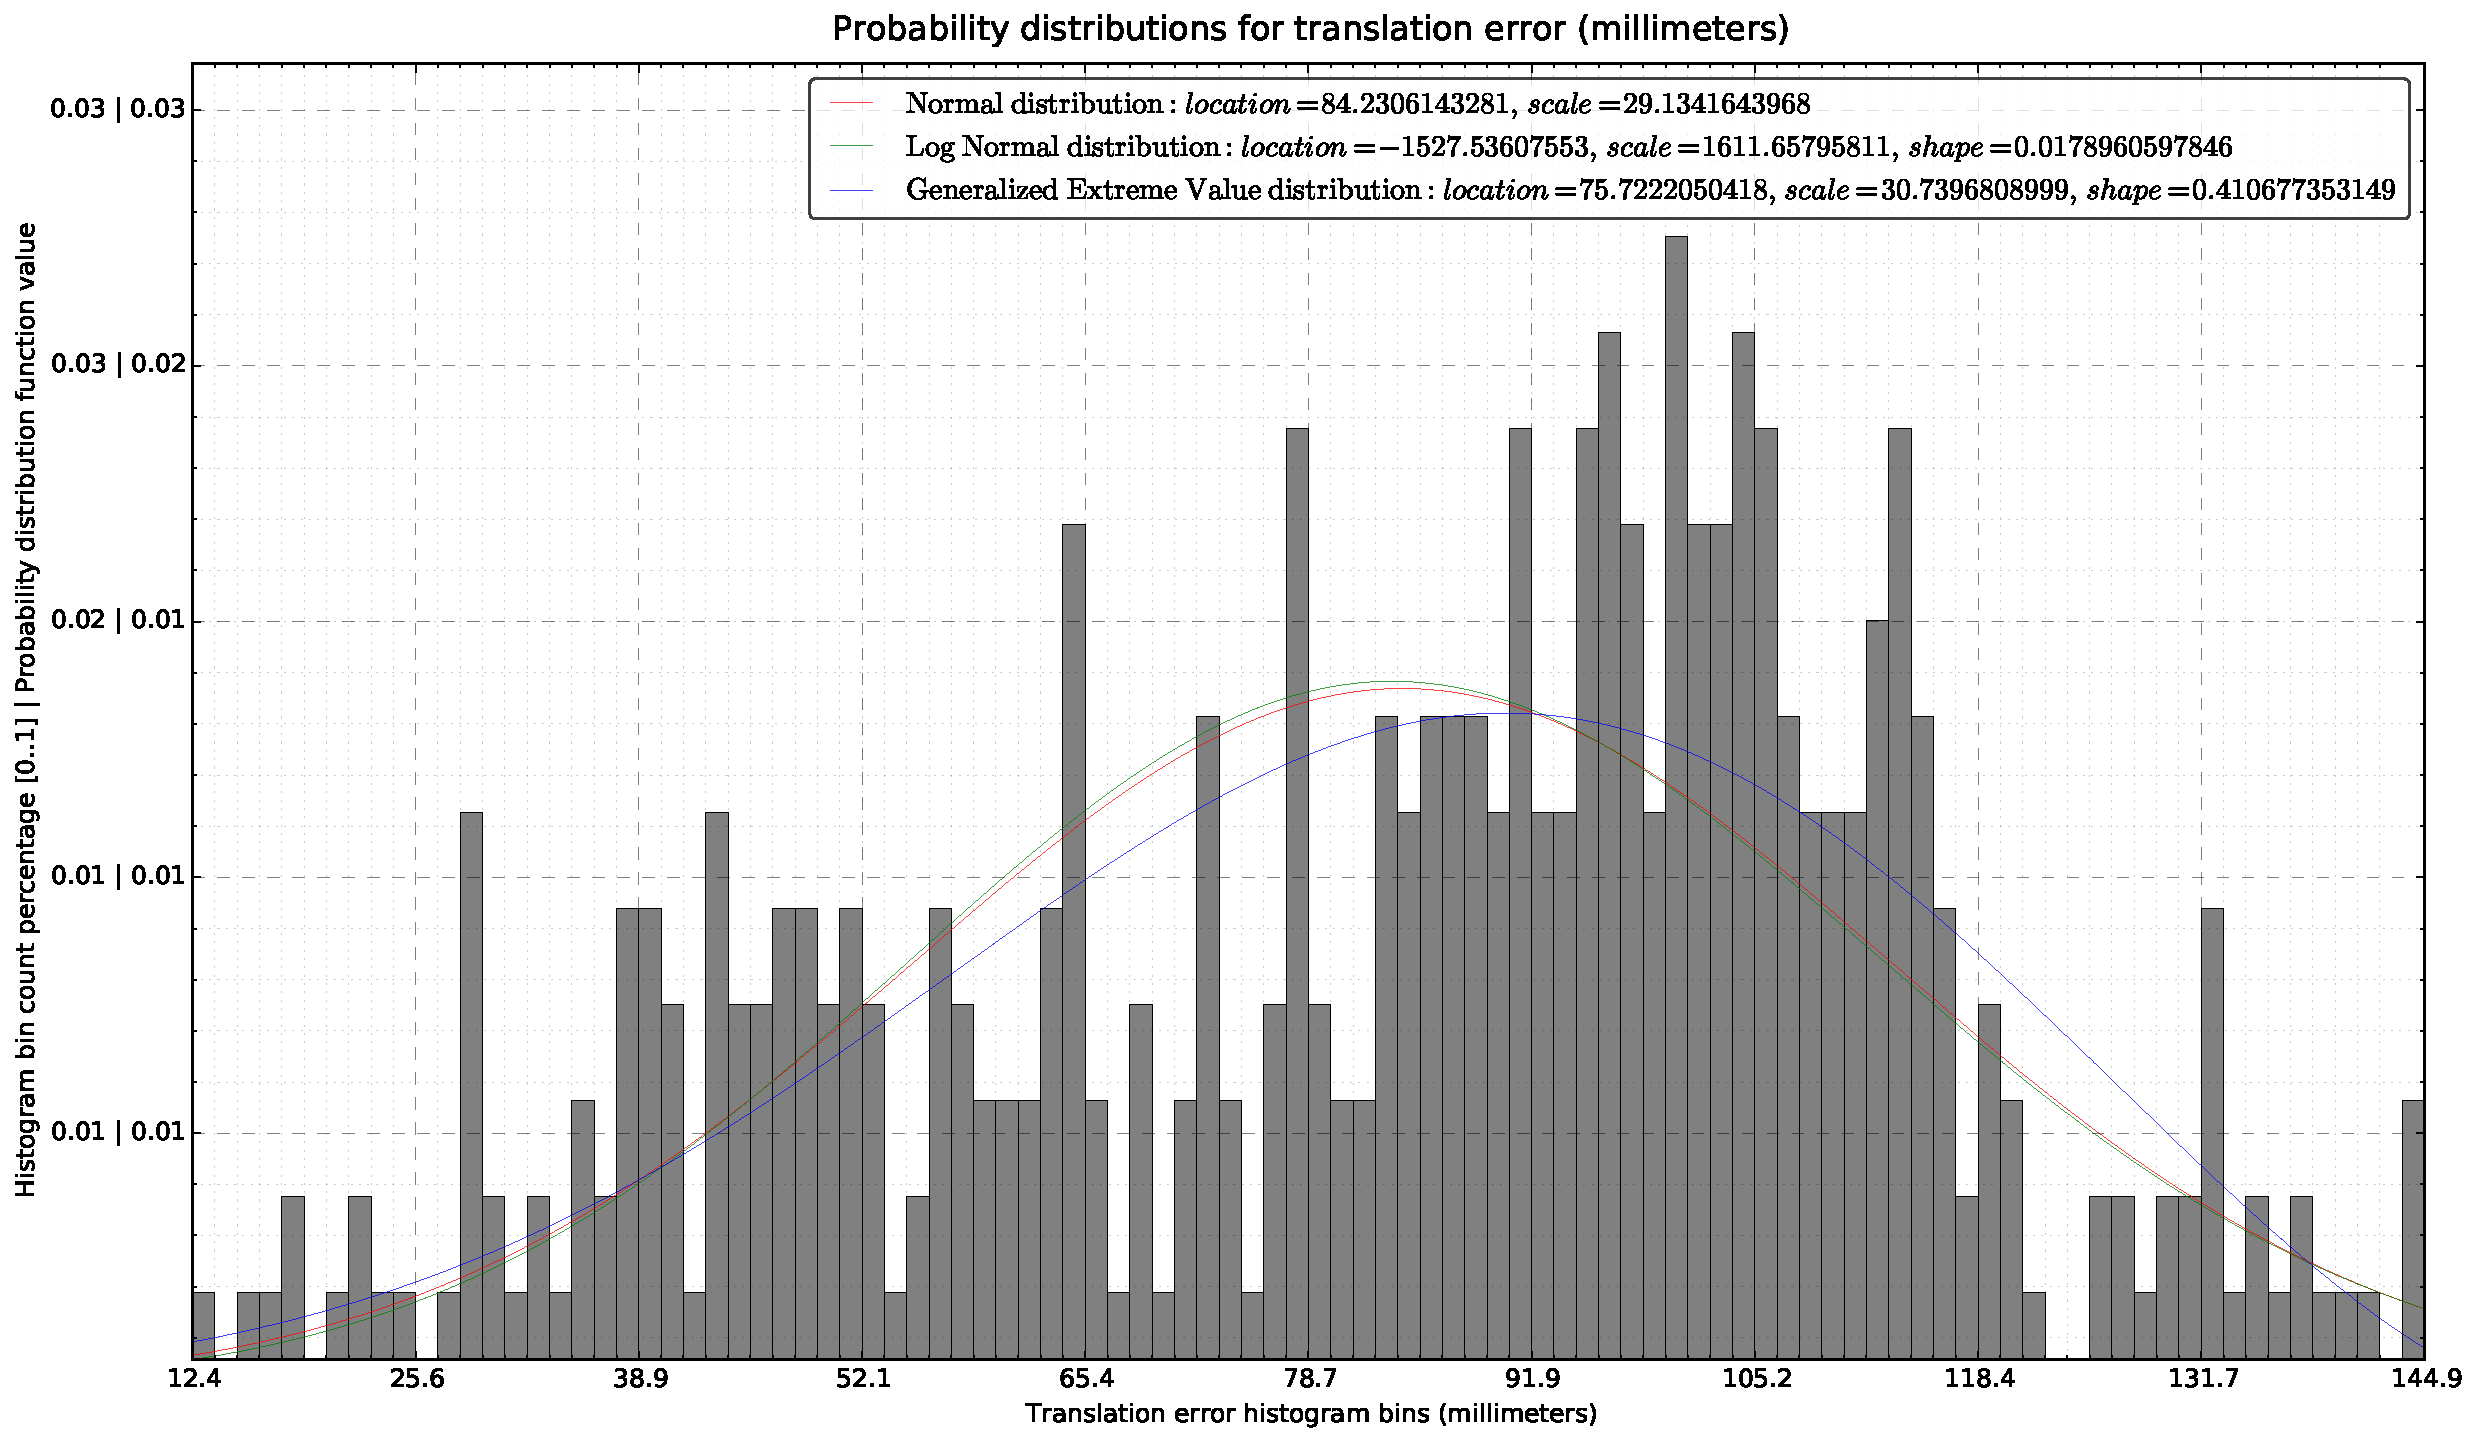
\includegraphics[width=0.65\textwidth]{localization-system-evaluation/tests-3dof/jarvis-robot/complex-path-with-outliers-50-30-50-10cm-per-sec-velocity-1-4-scans/graphs/translation-error-millimeters-distributions-amcl}
		\caption{Probability distributions for the \glsentrytext{amcl} translation errors}
		\label{fig:localization-system-evaluation_complex-path-with-outliers-50-30-50-10cm-per-sec-velocity-1-4-translation-error-amcl}
	\end{minipage}\hfill
	\begin{minipage}[H]{0.47\textwidth}
		\centering
		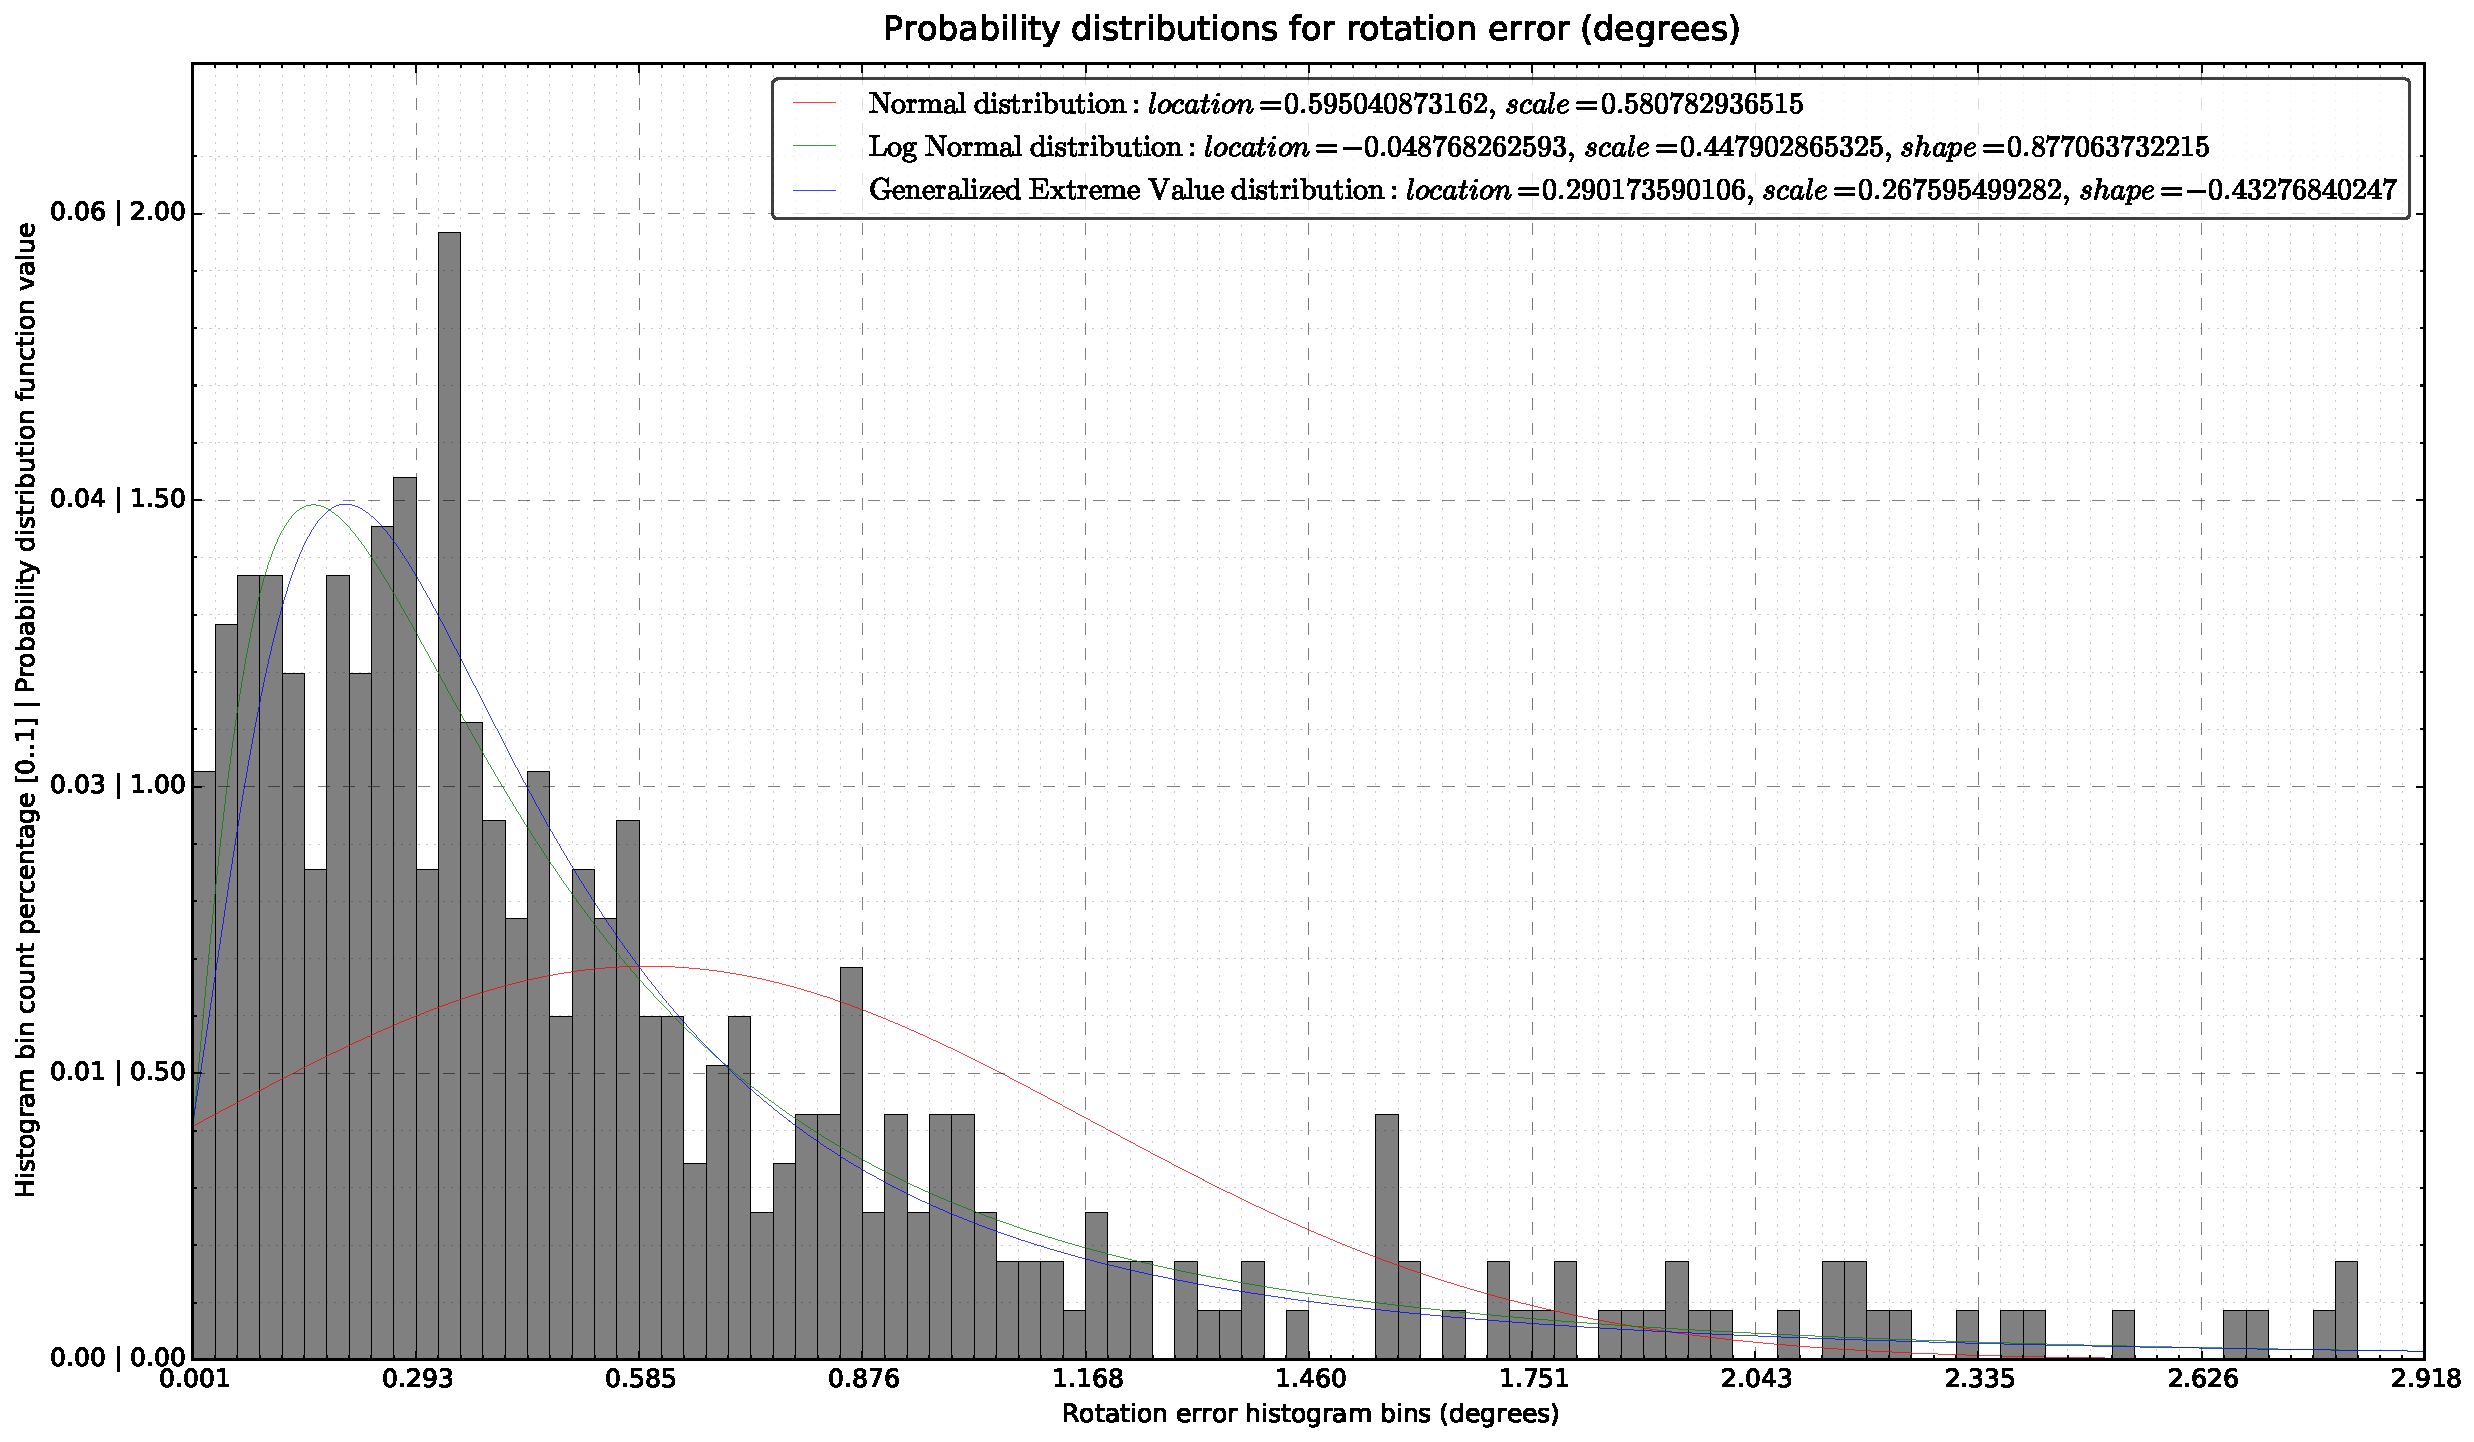
\includegraphics[width=0.65\textwidth]{localization-system-evaluation/tests-3dof/jarvis-robot/complex-path-with-outliers-50-30-50-10cm-per-sec-velocity-1-4-scans/graphs/rotation-error-degrees-distributions-amcl}
		\caption{Probability distributions for the \glsentrytext{amcl} rotation errors}
		\label{fig:localization-system-evaluation_complex-path-with-outliers-50-30-50-10cm-per-sec-velocity-1-4-rotation-error-amcl}
	\end{minipage}
\end{figure}

\begin{figure}[H]
	\centering
	\begin{minipage}[H]{0.47\textwidth}
		\centering
		\includegraphics[width=0.9\textwidth]{localization-system-evaluation/tests-3dof/jarvis-robot/complex-path-with-outliers-50-30-50-10cm-per-sec-velocity-1-4-scans/graphs/translation-error-millimeters-distributions}
		\caption{Probability distributions for the localization system translation errors}
		\label{fig:localization-system-evaluation_complex-path-with-outliers-50-30-50-10cm-per-sec-velocity-1-4-translation-error}
	\end{minipage}\hfill
	\begin{minipage}[H]{0.47\textwidth}
		\centering
		\includegraphics[width=0.9\textwidth]{localization-system-evaluation/tests-3dof/jarvis-robot/complex-path-with-outliers-50-30-50-10cm-per-sec-velocity-1-4-scans/graphs/rotation-error-degrees-distributions}
		\caption{Probability distributions for the localization system rotation errors}
		\label{fig:localization-system-evaluation_complex-path-with-outliers-50-30-50-10cm-per-sec-velocity-1-4-rotation-error}
	\end{minipage}
\end{figure}



\subsection{Computation time}

Looking at the computation time graphs in \cref{tab:localization-system-evaluation_3-dof-results} it can be seen that the localization system can register the point clouds very fast (between 5 and 30 milliseconds), which is low enough to process all the incoming laser scans in real time (typically \glspl{lidar} generate scans every 100 milliseconds). Moreover, the computation time seems to be very stable, with occasional peaks due to laser deformation or varying percentage of outliers.

The global computation time is mostly associated with the point cloud registration stage, while the rest of it is due to normal estimation and point cloud preprocessing algorithms.

\begin{figure}[H]
	\centering
	\includegraphics[width=0.45\textwidth]{localization-system-evaluation/tests-3dof/jarvis-robot/complex-path-with-outliers-50-30-50-10cm-per-sec-velocity-1-4-scans/graphs/computation-times-milliseconds-global-time-distributions}
	\caption{Probability distributions for the localization system global computation time}
	\label{fig:localization-system-evaluation_complex-path-with-outliers-50-30-50-10cm-per-sec-velocity-1-4-scans-computation-time}
\end{figure}



\clearpage

\section{6 \glsentrytext{dof} localization system tests}\label{sec:tridimensional-localization-system-tests}

\subsection{Overview}

The main 6 \gls{dof} results retrieved with the localization system are shown in \cref{tab:localization-system-evaluation_6-dof-results}. The first two experiments were done to evaluate the accuracy of the point cloud registration algorithms while the last one aimed to test the robustness against temporary absence of valid sensor data (in this test the Kinect had periods in which most of its field of view was outside the map).

These tests were retrieved with a known initial pose and used \gls{icp} point-to-point as tracking algorithm and \gls{icp} point-to-plane as tracking recovery method. The 3D map was done with the localization system in \gls{slam} mode and used continuous surface reconstruction in order to create an accurate representation of the environment and reduce the impact of the measurements noise. This map was later downsampled using a voxel grid with 20 mm cells in order to allow real-time processing of the Kinect data.

The next sections will provide an analysis of the 6 \gls{dof} results achieved with the proposed localization system. It will start by explaining the importance of point cloud processing and how it helps reduce the cloud registration time. Then it will give an overview of the 3D map building capabilities and it will finish with an analysis of the translation and rotation errors along with the computation time.


\begin{sidewaystable}
	\caption{6 \glsentrytext{dof} results}
	\tabulinesep = 1.2ex
	\setlength{\tabcolsep}{0.2em}
	\centering
	\tiny
	\begin{tabu} to \textwidth { X[m,c] X[1.7m,c] X[m,c] X[0.01m,c] X[m,c] X[m,c] X[0.01m,c] X[m,c] X[m,c] X[0.01m,c] X[m,c] X[m,c] X[0.01m,c] X[m,c] X[m,c] }
		\hline
		\multicolumn{3}{c}{Test conditions} && \multicolumn{2}{c}{Translation error (millimeters)} && \multicolumn{2}{c}{Rotation error (degrees)} && \multicolumn{2}{c}{Outliers percentage [0..100]} && \multicolumn{2}{c}{Global computation time (milliseconds)} \\
		\cline{1-3} \cline{5-6} \cline{8-9} \cline{11-12} \cline{14-15}
		Path shape 											& Path velocities 		& Map cell resolution 	&& Mean   	& Standard deviation 	&& Mean  	& Standard deviation 	&& Mean  	& Standard deviation 	&& Mean   & Standard deviation  \\ \hline
		Overview fly										& 30 cm/s				& 20 mm					&& 17.926	& 9.789					&& 3.027 	& 0.638					&& 0.165	& 0.172					&& 30.714 &	11.407				\\
		Mainly translations									& 20 cm/s				& 20 mm					&& 14.162	& 7.990					&& 2.486 	& 0.975					&& 0.983	& 1.874					&& 32.296 &	10.757				\\
		Mainly rotations									& 10 cm/s				& 20 mm					&& 16.576	& 9.389					&& 2.738 	& 0.583					&& 1.214	& 3.148					&& 29.818 &	9.134				\\
		\hline
	\end{tabu}
	\label{tab:localization-system-evaluation_6-dof-results}
\end{sidewaystable}


\subsection{Point cloud preprocessing}

Point cloud preprocessing can have a very significant role when performing 6 \gls{dof} cloud registration for self-localization. This is due to real-time requirements and also because the computation time increases substantially when registering large point clouds. One way to control this problem is by preprocessing the point cloud with a voxel grid to adjust the level of detail and also assign a limit to the number of points that come from sensors. This can be achieved with random sampling or similar point selection techniques, as can be seen in \cref{fig:localization-system-evaluation_kinect-fly-30cm-per-sec-velocity-drl-filters} (filtered cloud has larger points than the reference cloud). Moreover, depending on the sensor used, it may be wise to restrict the points to a given range, and discard the rest that are too far way (given that these measurements will have more errors).

\begin{figure}[H]
	\centering
	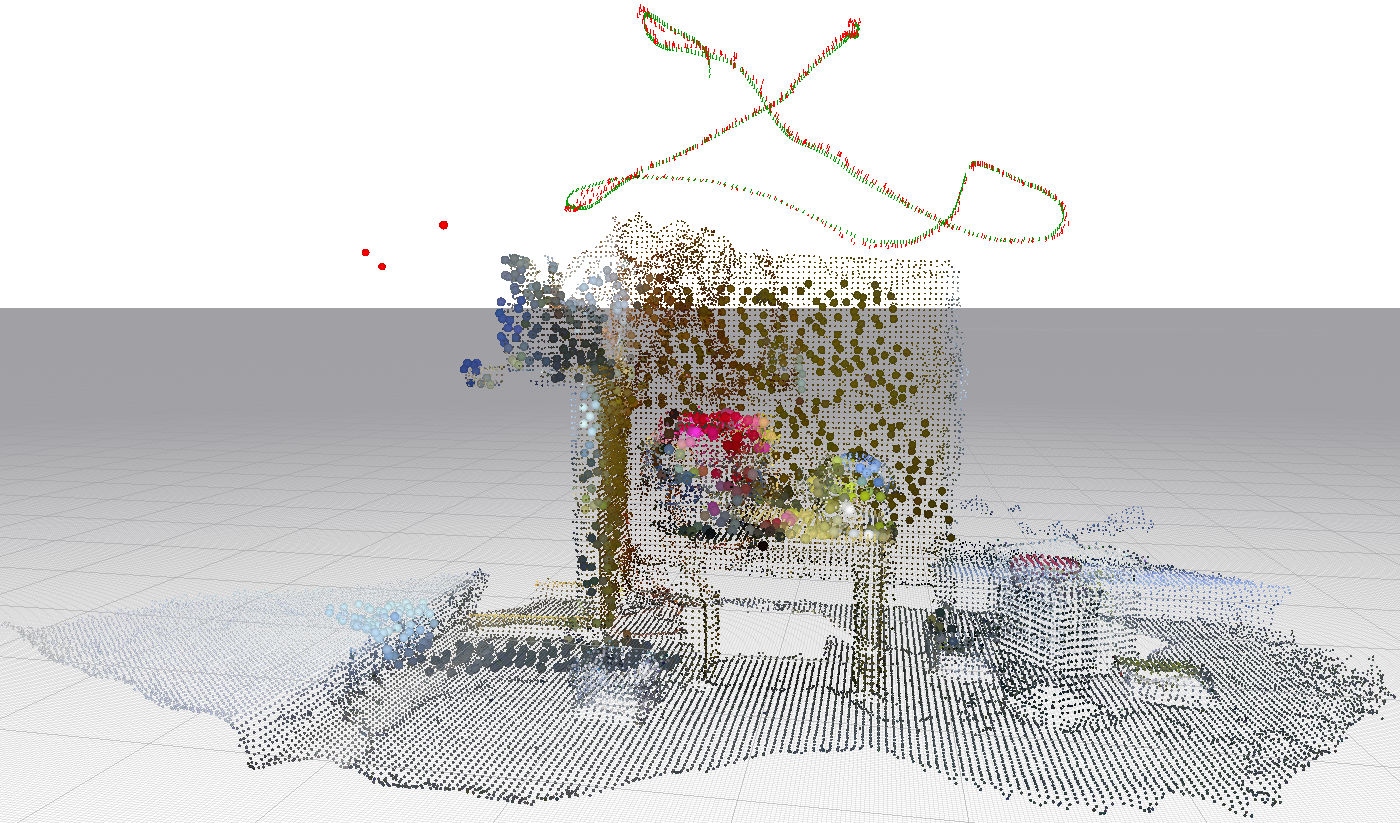
\includegraphics[width=0.45\textwidth]{localization-system-evaluation/tests-6dof/kinect-fly-30cm-per-sec-velocity/drl}
	\caption{Example of filtered point cloud from Kinect data}
	\label{fig:localization-system-evaluation_kinect-fly-30cm-per-sec-velocity-drl-filters}
\end{figure}


\subsection{\glsentrytext{slam}}

The proposed localization system can perform mapping of the environment and is able to build very detailed point clouds. These point clouds can be continuously re-sampled with the Moving Least Squares algorithm (example in \cref{fig:localization-system-evaluation_kinect-fly-30cm-per-sec-velocity-drl-slam}) in order to reconstruct the surfaces of the environment and attenuate the double wall effects and high sensor noise.

The localization system can also dynamic update the 3D map in order to remove missing objects from the reference point cloud and also add new ones.


\begin{figure}[H]
	\centering
	\begin{subfigure}[ht]{0.45\textwidth}
		\centering
		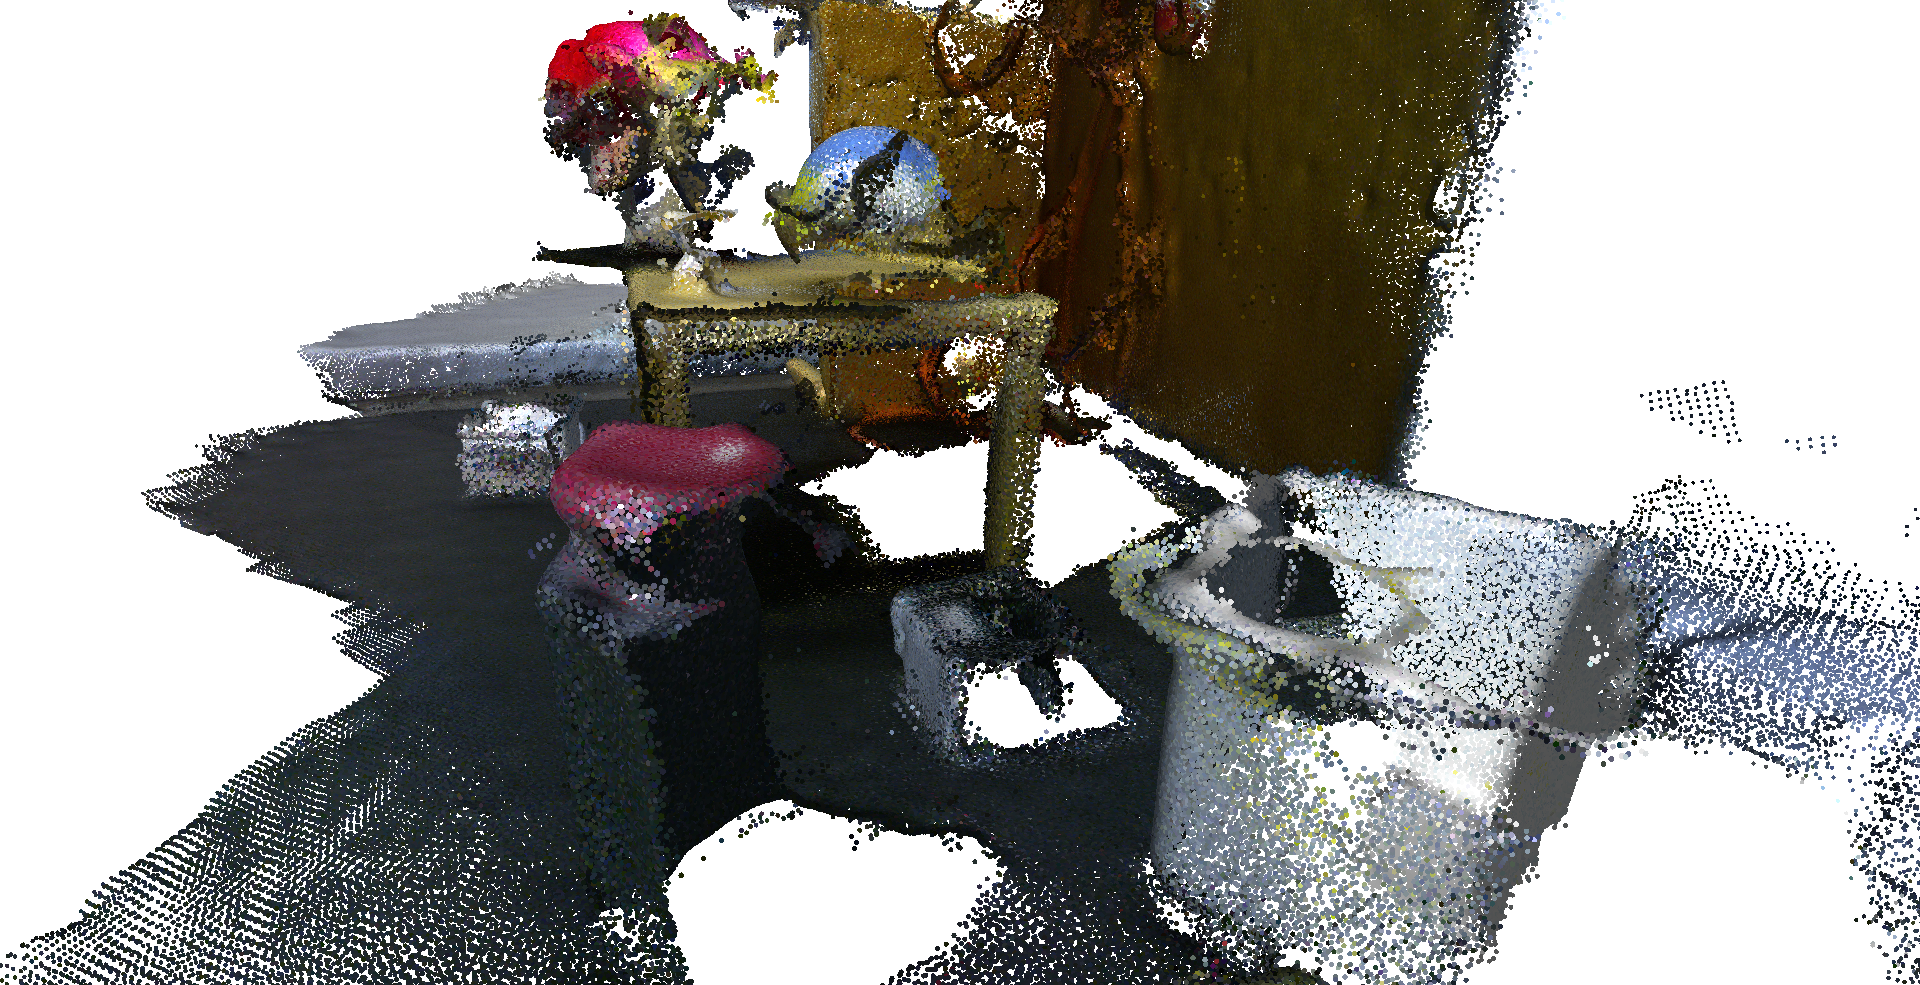
\includegraphics[width=\textwidth]{localization-system-evaluation/tests-6dof/kinect-fly-30cm-per-sec-velocity/3d-slam-1}
	\end{subfigure}
	\begin{subfigure}[ht]{0.45\textwidth}
		\centering
		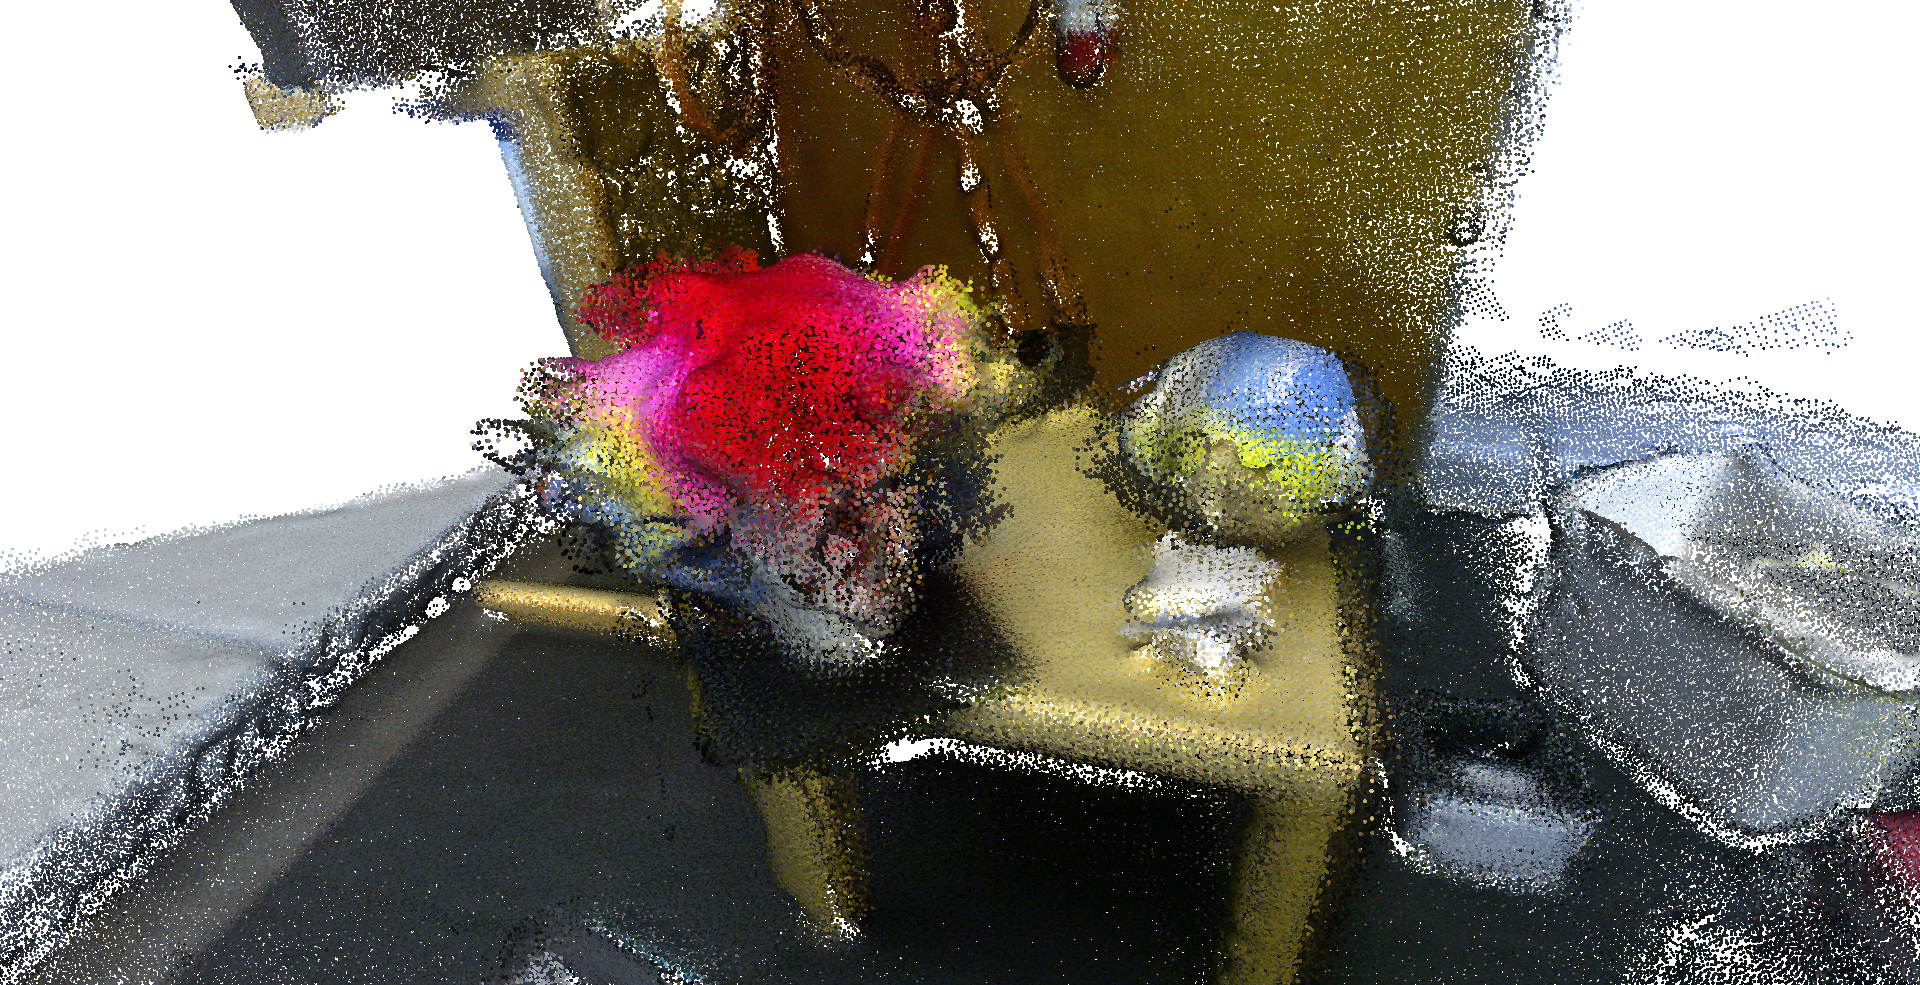
\includegraphics[width=\textwidth]{localization-system-evaluation/tests-6dof/kinect-fly-30cm-per-sec-velocity/3d-slam-2}
	\end{subfigure}
	\begin{subfigure}[ht]{0.45\textwidth}
		\centering
		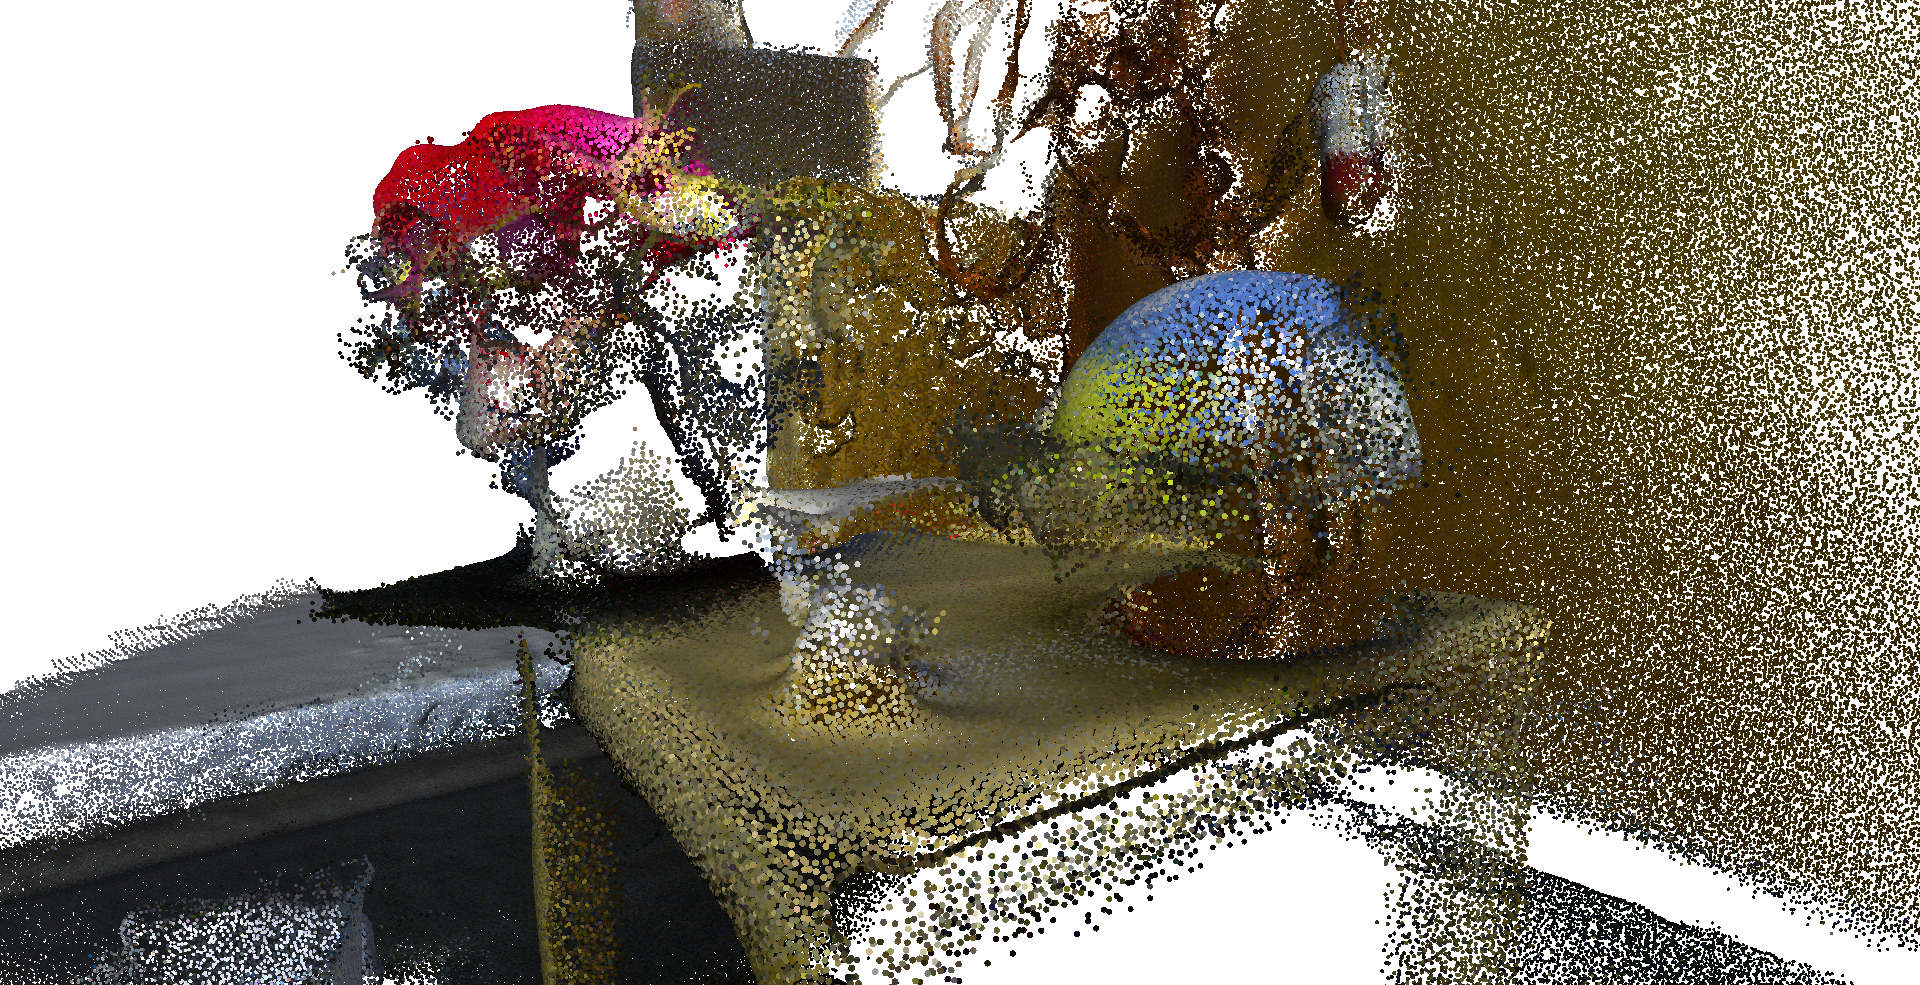
\includegraphics[width=\textwidth]{localization-system-evaluation/tests-6dof/kinect-fly-30cm-per-sec-velocity/3d-slam-3}
	\end{subfigure}
	\begin{subfigure}[ht]{0.45\textwidth}
		\centering
		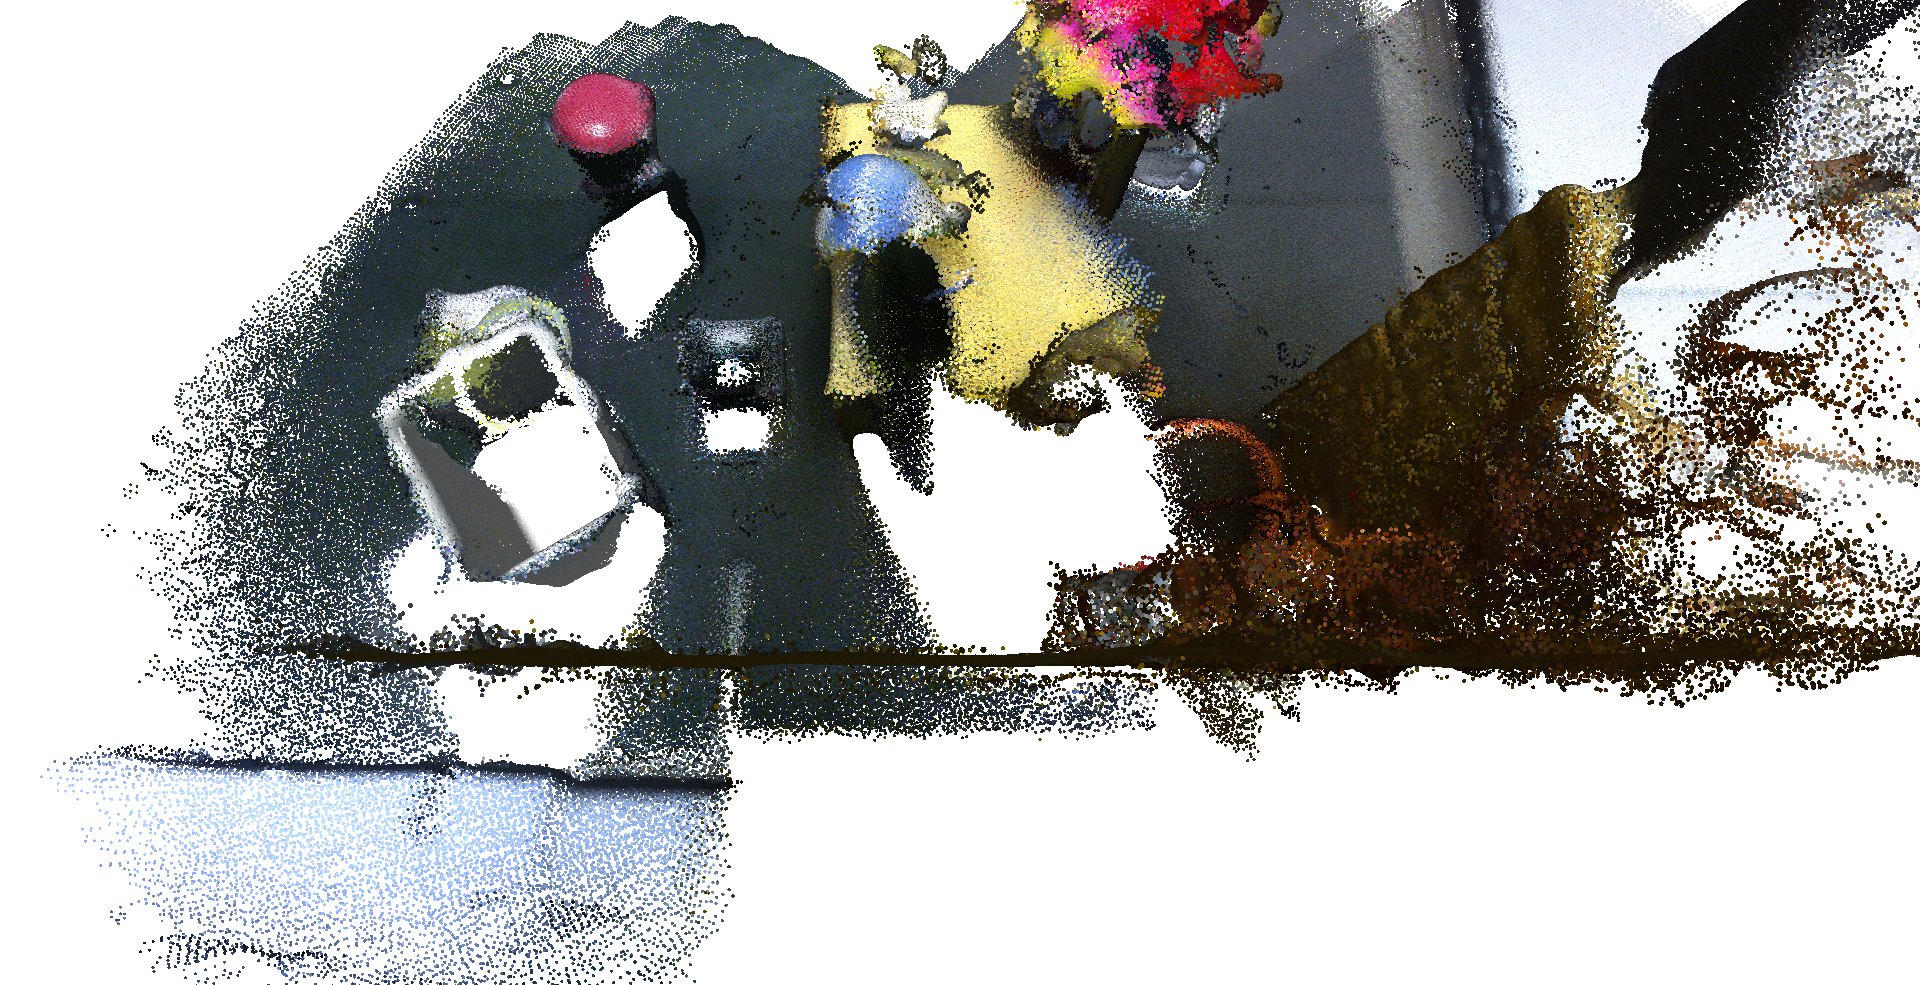
\includegraphics[width=\textwidth]{localization-system-evaluation/tests-6dof/kinect-fly-30cm-per-sec-velocity/3d-slam-4}
	\end{subfigure}
	\caption{3D SLAM using the localization system with surface reconstruction}
	\label{fig:localization-system-evaluation_kinect-fly-30cm-per-sec-velocity-drl-slam}
\end{figure}

\begin{figure}[H]
	\centering
	\begin{subfigure}[ht]{0.45\textwidth}
		\centering
		\includegraphics[width=\textwidth]{localization-system-evaluation/tests-6dof/kinect-fly-30cm-per-sec-velocity/3d-slam-1-gt}
	\end{subfigure}
	\begin{subfigure}[ht]{0.45\textwidth}
		\centering
		\includegraphics[width=\textwidth]{localization-system-evaluation/tests-6dof/kinect-fly-30cm-per-sec-velocity/3d-slam-2-gt}
	\end{subfigure}
	\begin{subfigure}[ht]{0.45\textwidth}
		\centering
		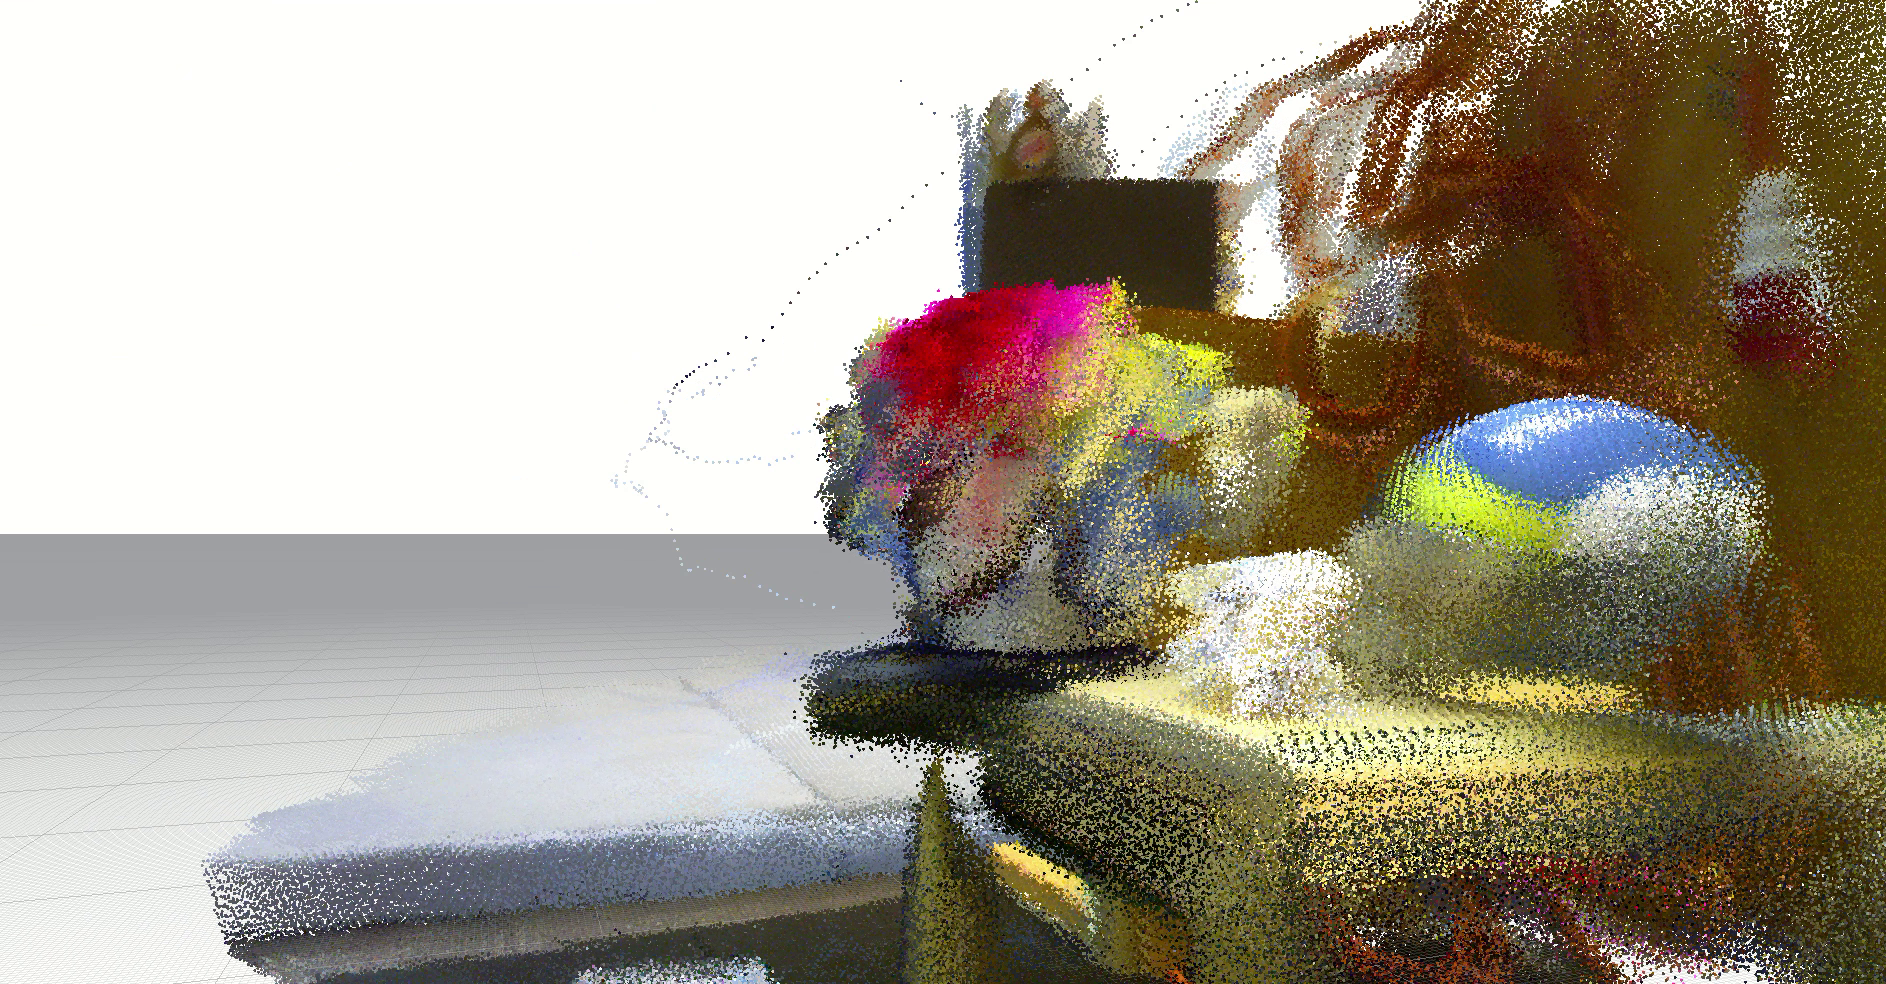
\includegraphics[width=\textwidth]{localization-system-evaluation/tests-6dof/kinect-fly-30cm-per-sec-velocity/3d-slam-3-gt}
	\end{subfigure}
	\begin{subfigure}[ht]{0.45\textwidth}
		\centering
		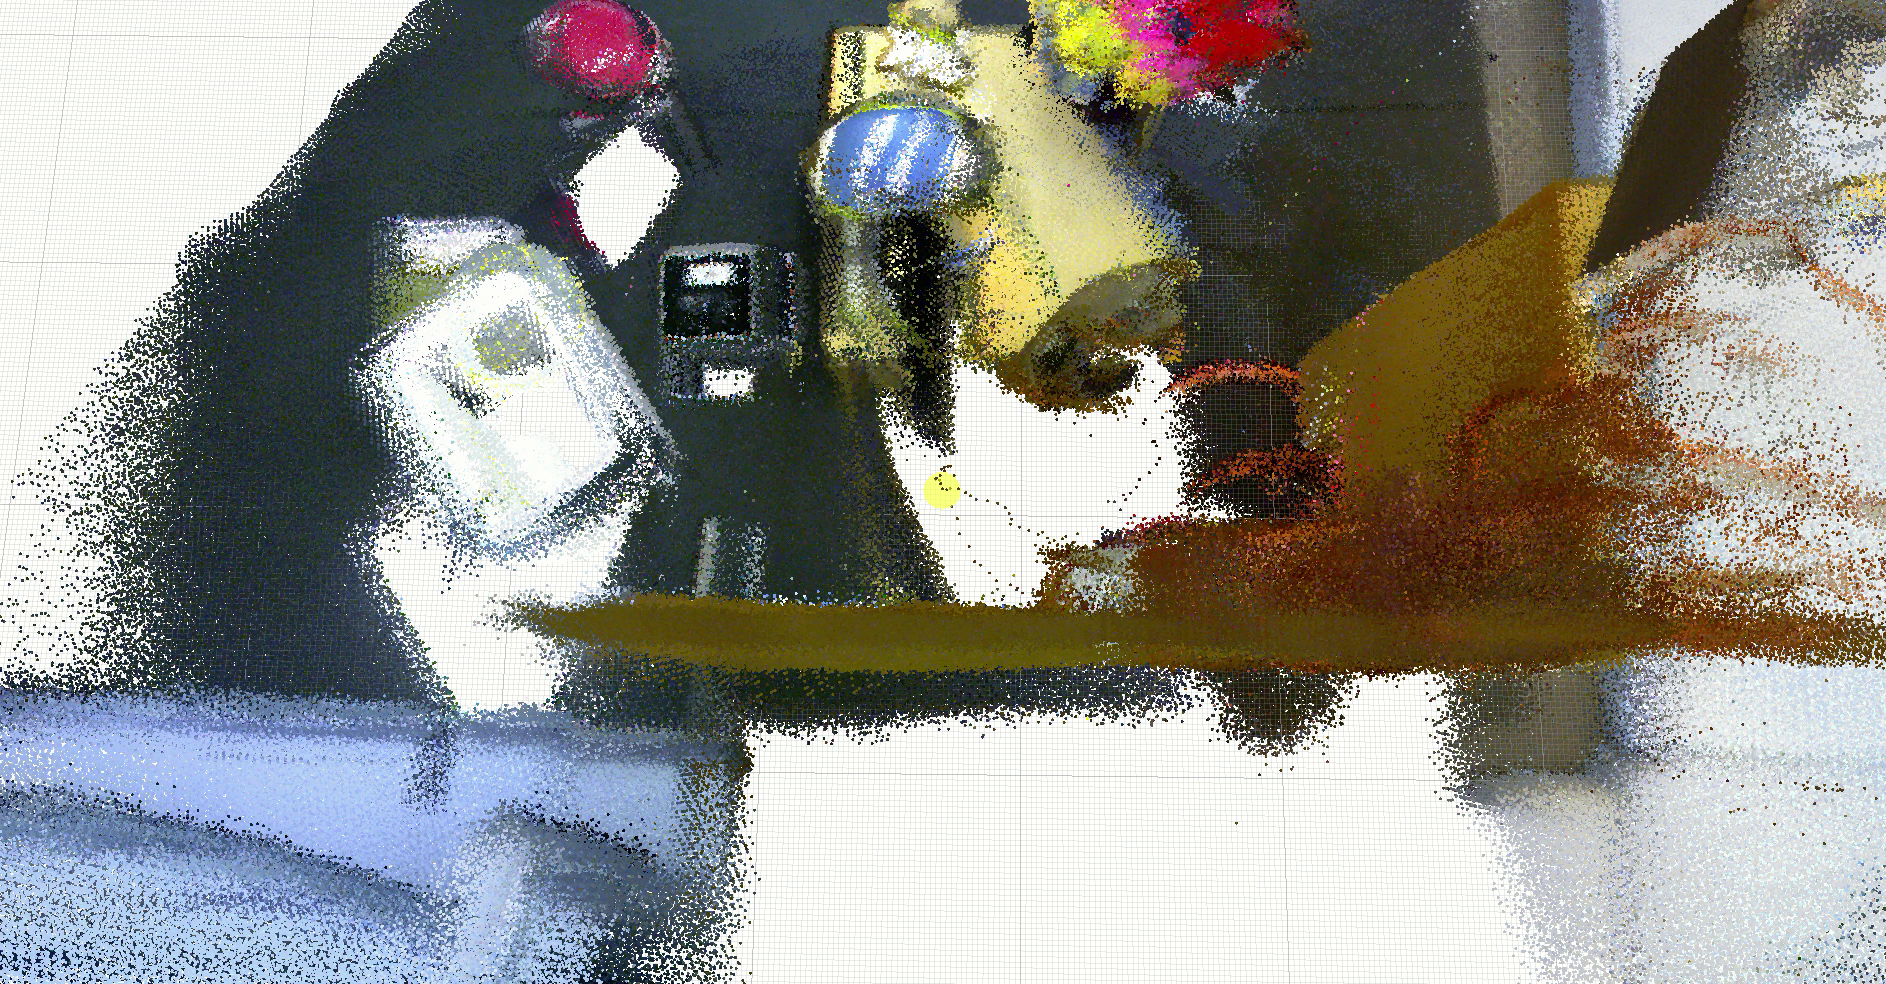
\includegraphics[width=\textwidth]{localization-system-evaluation/tests-6dof/kinect-fly-30cm-per-sec-velocity/3d-slam-4-gt}
	\end{subfigure}
	\caption{3D SLAM using the ground truth poses}
	\label{fig:localization-system-evaluation_kinect-fly-30cm-per-sec-velocity-gt-slam}
\end{figure}


\subsection{Point cloud registration}

Looking at \cref{tab:localization-system-evaluation_6-dof-results} and the assembly of the registered point clouds (shown in \cref{fig:localization-system-evaluation_kinect-fly-30cm-per-sec-velocity-drl-cumulative}), it is clear that the proposed localization system is able to register point clouds with high accuracy, even when they are severely downsampled (due to real-time processing constraints). Moreover, the localization system is robust against temporary absence of sensor data (when the field of view of the Kinect was outside the known map) and was able to quickly recover to accurate tracking when valid sensor data was given. In these situations the recovery algorithms were activated, switching the registration algorithm from \gls{icp} point-to-point to \gls{icp} point-to-plane. Given that these sensor data outages were temporary, the initial pose algorithms weren't necessary. Nevertheless, if the Kinect remained outside the map for a longer period of time, the localization system would alert that the tracking was lost and it would try to find its current pose using feature matching.

Comparing \cref{fig:localization-system-evaluation_kinect_translation_path} and \cref{fig:localization-system-evaluation_kinect_translation_path2}, it can be seen that the proposed localization system achieved better pose tracking than the \emph{ethzasl\_icp\_mapper} \gls{ros} package \cite{Pomerleau2011} (authors of this Kinect dataset). Moreover, the \gls{slam} map shown in \cref{fig:localization-system-evaluation_kinect-fly-30cm-per-sec-velocity-drl-slam} seems to have better quality than the map generated using the ground truth poses (shown in \cref{fig:localization-system-evaluation_kinect-fly-30cm-per-sec-velocity-gt-slam,fig:localization-system-evaluation_kinect-fly-30cm-per-sec-velocity-gt-cumulative}).

\begin{figure}[H]
	\centering
	\begin{minipage}[b]{0.24\textwidth}
		\centering
		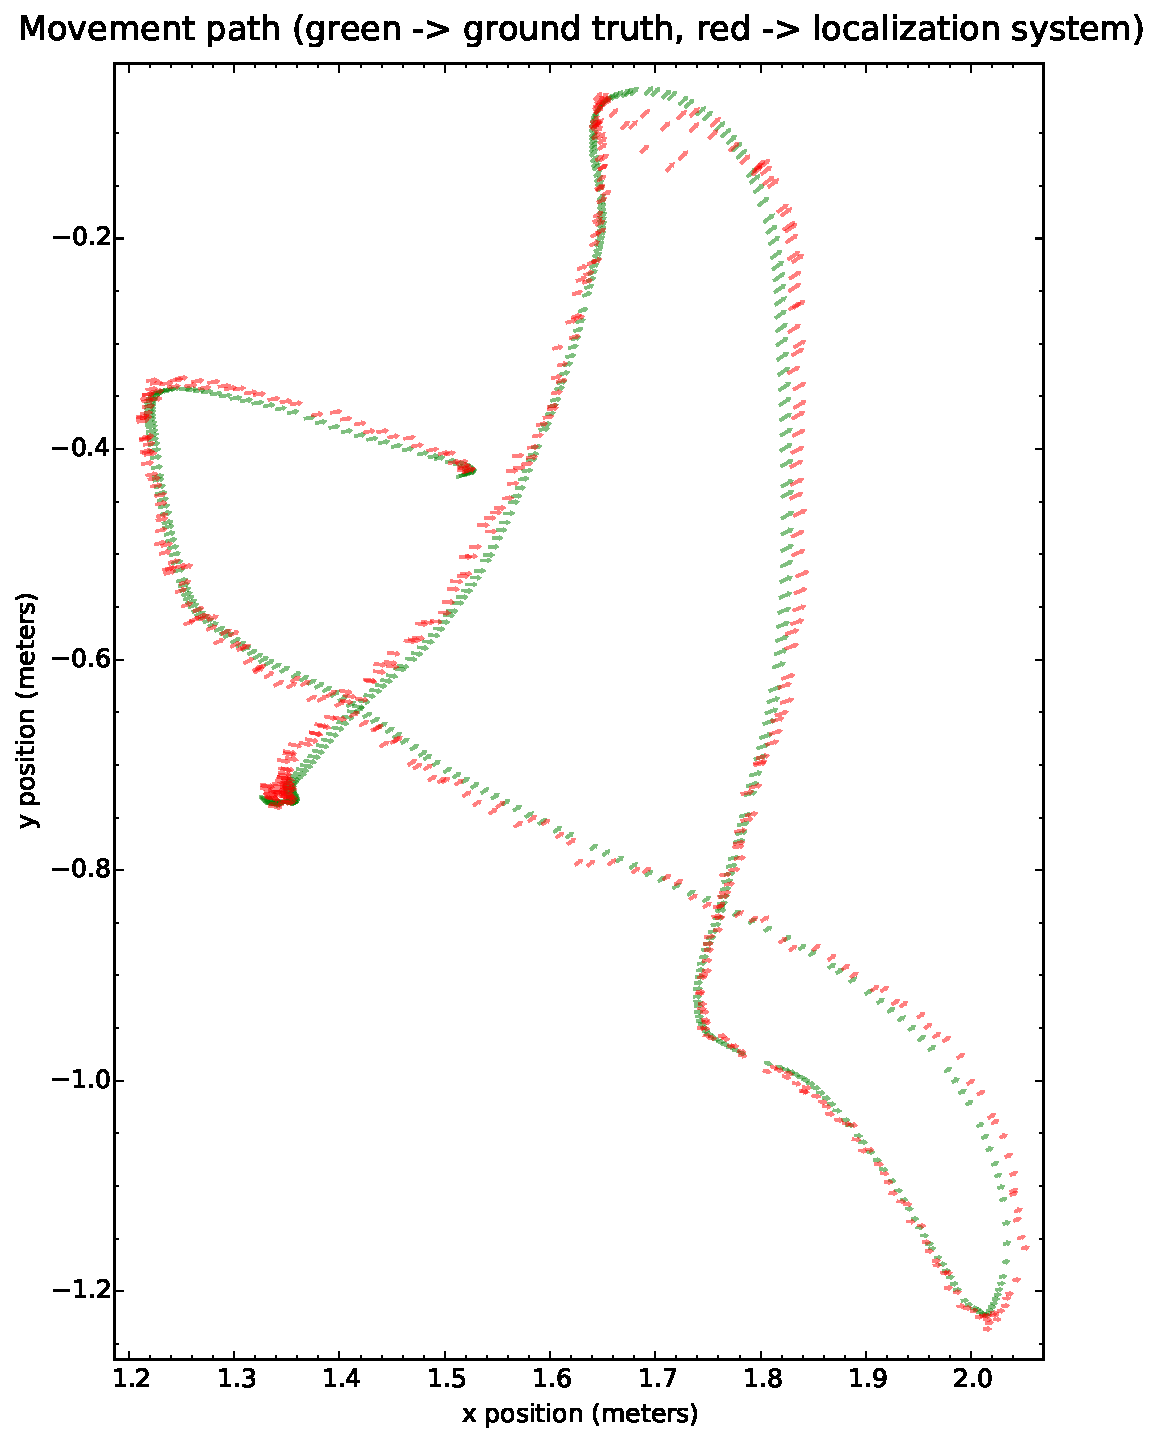
\includegraphics[width=0.97\textwidth]{localization-system-evaluation/tests-6dof/kinect-fly-30cm-per-sec-velocity/robot-movement-path}
		\caption{Poses estimated by the ground truth and localization system}
		\label{fig:localization-system-evaluation_kinect_translation_path}
	\end{minipage}\hfill
	\begin{minipage}[b]{0.24\textwidth}
		\centering
		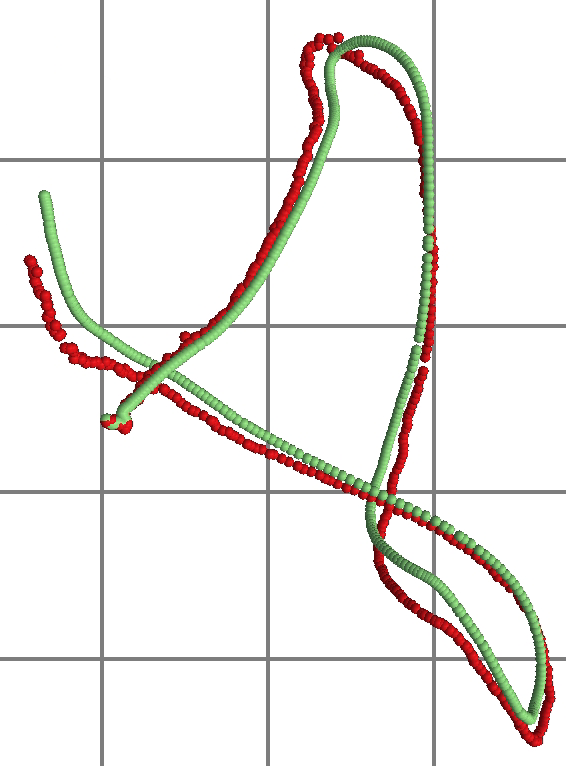
\includegraphics[width=0.8\textwidth]{localization-system-evaluation/tests-6dof/kinect-fly-30cm-per-sec-velocity/ethzasl-icp-mapping-path}
		\caption{Poses estimated by the \emph{ethzasl\_icp\_mapper} \glsentrytext{ros} package \cite{Pomerleau2011}}
		\label{fig:localization-system-evaluation_kinect_translation_path2}
	\end{minipage}
\end{figure}

\begin{figure}[H]
	\centering
	\includegraphics[width=0.37\textwidth]{localization-system-evaluation/tests-6dof/kinect-fly-30cm-per-sec-velocity/drl-cumulative}
	\caption{Point clouds assembled on top of the map using the localization system poses (for the top part of the figure: green arrows $\rightarrow$ ground truth poses, red arrows $\rightarrow$ localization system poses)}
	\label{fig:localization-system-evaluation_kinect-fly-30cm-per-sec-velocity-drl-cumulative}
\end{figure}

\begin{figure}[H]
	\centering
	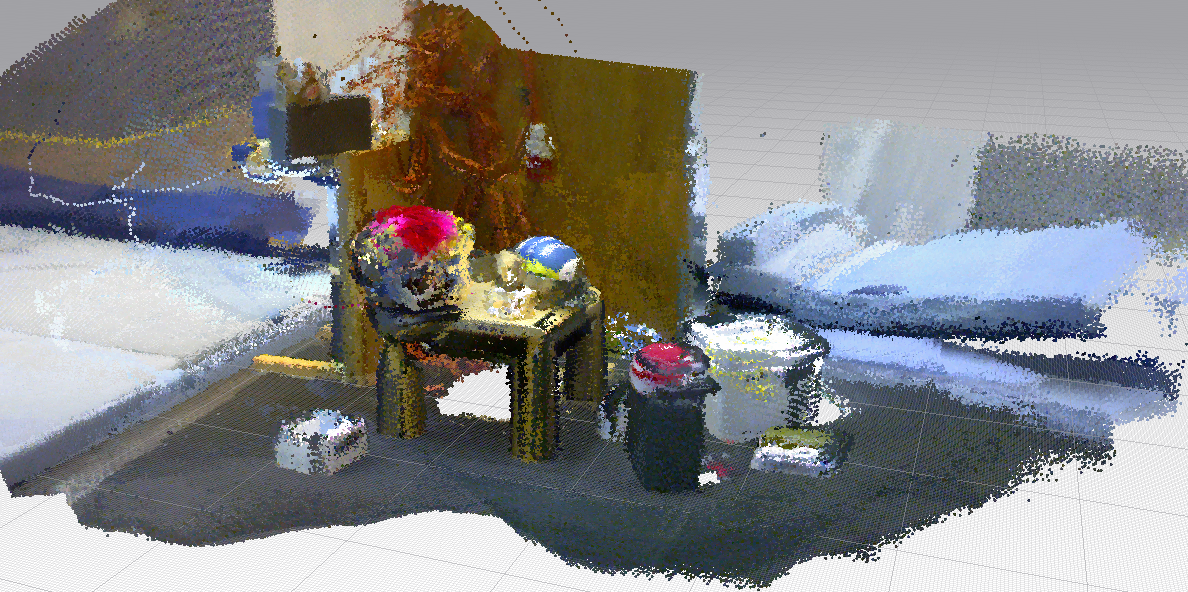
\includegraphics[width=0.37\textwidth]{localization-system-evaluation/tests-6dof/kinect-fly-30cm-per-sec-velocity/ground-truth-cumulative}
	\caption{Point clouds assembled on top of the map using the ground truth poses}
	\label{fig:localization-system-evaluation_kinect-fly-30cm-per-sec-velocity-gt-cumulative}
\end{figure}


\subsection{Translation and rotation errors}

The results presented in \cref{tab:localization-system-evaluation_6-dof-results} and in \cref{fig:localization-system-evaluation_kinect-fly-30cm-per-sec-velocity-translation-error,fig:localization-system-evaluation_kinect-fly-30cm-per-sec-velocity-rotation-error}, shown that the localization system can maintain high accuracy pose tracking, with translation error bellow two centimeters and rotation error around 3 degrees when good sensor data is available. Moreover it can quickly recover from temporary registration problems caused by occlusions or accelerations.

\Cref{fig:localization-system-evaluation_kinect_translation_path,fig:localization-system-evaluation_kinect_translation_path2} also shows that the proposed localization system achieved less overall translation error than the tracking system proposed by the authors of this Kinect dataset \cite{Pomerleau2011}.


\begin{figure}[H]
	\centering
	\begin{minipage}[H]{0.45\textwidth}
		\centering
		\includegraphics[width=0.75\textwidth]{localization-system-evaluation/tests-6dof/kinect-fly-30cm-per-sec-velocity/translation-error-millimeters-distributions}
		\caption{Probability distributions for the localization system translation errors}
		\label{fig:localization-system-evaluation_kinect-fly-30cm-per-sec-velocity-translation-error}
	\end{minipage}\hfill
	\begin{minipage}[H]{0.45\textwidth}
		\centering
		\includegraphics[width=0.75\textwidth]{localization-system-evaluation/tests-6dof/kinect-fly-30cm-per-sec-velocity/rotation-error-degrees-distributions}
		\caption{Probability distributions for the localization system rotation errors}
		\label{fig:localization-system-evaluation_kinect-fly-30cm-per-sec-velocity-rotation-error}
	\end{minipage}
\end{figure}


\subsection{Computation time}

The localization system was able to achieve a mean computation time low enough to allow real time processing of the Kinect point cloud sensor data (shown in \cref{fig:localization-system-evaluation_kinect-fly-30cm-per-sec-velocity-computation-time}). Depending on the accuracy requirements, the computation time can be lowered even further by tuning the preprocessing filters, in order to reduce the number of points used in the cloud registration.

\begin{figure}[H]
	\centering
	\includegraphics[width=0.35\textwidth]{localization-system-evaluation/tests-6dof/kinect-fly-30cm-per-sec-velocity/computation-times-milliseconds-global-time-distributions}
	\caption{Probability distributions for the localization system global computation time}
	\label{fig:localization-system-evaluation_kinect-fly-30cm-per-sec-velocity-computation-time}
\end{figure}
